\documentclass[12pt, a4paper]{article}

% --- Packages ---
\usepackage[utf8]{inputenc}
\usepackage[T1]{fontenc}
\usepackage{geometry}
\geometry{a4paper, margin=1in, headheight=15pt}
\usepackage{xcolor}
\usepackage{hyperref}
\usepackage{graphicx}
\usepackage{tcolorbox}
\usepackage{fancyhdr}
\usepackage{titlesec}
\usepackage{enumitem}
\usepackage{parskip}
\usepackage{caption}
\usepackage{float}
\usepackage{listings}

% --- Colors ---
\definecolor{primary}{RGB}{12, 74, 110}     % Dark Slate Blue
\definecolor{secondary}{RGB}{2, 132, 199}   % Sky Blue
\definecolor{accent}{RGB}{240, 249, 255}    % Very Light Blue for backgrounds
\definecolor{darkgray}{RGB}{71, 85, 105}
\definecolor{codebg}{RGB}{248, 250, 252}

% --- Hyperref Setup ---
\hypersetup{
    colorlinks=true,
    linkcolor=primary,
    filecolor=secondary,      
    urlcolor=secondary,
    pdftitle={Comprehensive Week 3 Report - CalderR Internship},
    pdfpagemode=FullScreen,
}

% --- Header and Footer Setup ---
\pagestyle{fancy}
\fancyhf{}
\rhead{\textcolor{darkgray}{\textbf{Week 3 Comprehensive Report}}}
\lhead{\textcolor{darkgray}{CalderR Agentic AI Internship, 2026}}
\cfoot{\textcolor{darkgray}{Page \thepage}}
\renewcommand{\headrulewidth}{0.4pt}
\renewcommand{\footrulewidth}{0.4pt}

% --- Section Formatting ---
\titleformat{\section}
  {\LARGE\bfseries\color{primary}}{\thesection}{1em}{}[{\titlerule[1.2pt]}]

\titleformat{\subsection}
  {\Large\bfseries\color{secondary}}{\thesubsection}{1em}{}

\titleformat{\subsubsection}
  {\large\bfseries\color{primary}}{\thesubsubsection}{1em}{}

% --- Document Starts Here ---
\begin{document}

% --- Title Page ---
\begin{titlepage}
    \centering
    \vspace*{2cm}
    
    {\Huge \textbf{\textcolor{primary}{Agentic AI Engineering Internship}}} \\[0.5cm]
    {\Huge \textbf{\textcolor{primary}{2026}}} \\[1.5cm]
    
    {\LARGE \textbf{Week 3 Comprehensive Report}} \\[0.5cm]
    {\Large \textit{Embeddings, RAG \& Vector Databases}} \\[2cm]
    
    \begin{tcolorbox}[colback=accent, colframe=primary, rounded corners, boxrule=1.5pt, width=0.75\textwidth, arc=4mm]
        \centering
        \vspace{0.4cm}
        {\Large \textbf{Prepared By:}} \\[0.2cm]
        {\Large \textbf{Ghafoor}} \\[0.4cm]
        {\large \textbf{Date:}} \\
        {\large \today}
        \vspace{0.4cm}
    \end{tcolorbox}
    
    \vfill
    
    {\huge \textbf{\textcolor{secondary}{CalderR.}}} \\[0.2cm]
    {\large \textit{RETHINKING $\cdot$ HOW $\cdot$ WORK $\cdot$ WORKS}}
    \vspace*{1cm}
\end{titlepage}

% --- Table of Contents ---
\tableofcontents
\newpage

% --- Section 1: Executive Summary ---
\section{Executive Summary}
This comprehensive report documents the theoretical learnings, hands-on labs, and advanced architectural implementations completed during Week 3 of the CalderR Agentic AI Engineering Internship. Building upon the prompt engineering and tool-calling mechanics established previously, the core objective of this week was to master Retrieval-Augmented Generation (RAG) at scale. The week introduced the foundational technologies that allow AI systems to reason over external knowledge they were never trained on, focusing heavily on vector embeddings, vector databases, and sophisticated retrieval architectures.

The week culminated in the successful deployment of two complex projects: a \textbf{Personal Knowledge Base} (Intermediate) and an \textbf{Enterprise Document Intelligence Platform} (Production). These projects synthesized the week's learnings by implementing multi-tenant data ingestion pipelines, hybrid search mechanisms (BM25 + Semantic), cross-encoder re-ranking for enhanced accuracy, and rigorous evaluation using the RAGAS framework.

% --- Section 2: Conceptual Mastery & Assessment ---
\section{Conceptual Mastery \& Assessment}
The curriculum emphasized transitioning from naive generation into robust, fact-based AI systems via vector-based retrieval.

\subsection{Embeddings, RAG \& Vector Databases}
\begin{itemize}[label=\textcolor{secondary}{$\bullet$}]
    \item \textbf{Embeddings \& Semantic Search:} Explored the mathematical representation of textual meaning via high-dimensional vector spaces. Implemented cosine similarity metrics and compared local embedding models (e.g., \texttt{sentence-transformers}, \texttt{all-MiniLM-L6-v2}, and \texttt{bge-small-en}).
    \item \textbf{Vector Databases:} Mastered the storage, indexing, and querying of embeddings. Utilized ChromaDB and FAISS for efficient nearest-neighbor searches, focusing on the tradeoffs between in-memory structures and persistent server-based storage.
    \item \textbf{Advanced RAG Architecture:} Evolved beyond naive RAG (load $\rightarrow$ split $\rightarrow$ embed $\rightarrow$ retrieve $\rightarrow$ generate) by building sophisticated query pipelines. Implemented Hybrid Retrieval (Semantic + BM25 keyword search) utilizing LangChain's \texttt{EnsembleRetriever}, augmented by Cross-Encoder re-ranking to drastically improve top-k retrieval accuracy.
    \item \textbf{RAG Evaluation Frameworks:} Adopted an engineering mindset toward LLM evaluation. Integrated the RAGAS framework to quantitatively measure system performance across key metrics: \textit{faithfulness}, \textit{answer relevancy}, \textit{context precision}, and \textit{context recall}.
\end{itemize}

\newpage

% --- Section 3: Production Project ---
\section{Production Project: Enterprise Document Intelligence Platform}

\begin{tcolorbox}[colback=accent, colframe=primary, title=\textbf{Architectural Overview}, boxrule=1pt]
The flagship deliverable for Week 3 is a robust, multi-tenant Enterprise Document Intelligence Platform. Built using FastAPI and Streamlit, it allows users to securely upload, process, and query documents. The backend features asynchronous document processing, tenant-isolated ChromaDB collections, and an advanced RAG pipeline leveraging hybrid search and re-ranking to deliver highly accurate answers accompanied by confidence scores and source citations.
\end{tcolorbox}

\subsection{Technical Implementation}
\begin{itemize}[label=\textcolor{secondary}{$\bullet$}]
    \item \textbf{Multi-Tenant Async Backend:} Engineered a scalable FastAPI backend with background task workers (\texttt{asyncio}) handling heavy document chunking and embedding processes.
    \item \textbf{Tenant Isolation in Vector DB:} Dynamically namespaced ChromaDB collections ensure strict data isolation between different enterprise clients.
    \item \textbf{Advanced Retrieval Pipeline:} Executed a multi-stage retrieval architecture: a base Hybrid Search (BM25 + ChromaDB semantic search) followed by a BAAI \texttt{bge-reranker} to reorder the context chunks before LLM synthesis.
\end{itemize}

\subsection{System Demonstrations}
\begin{figure}[H]
    \centering
    \begin{minipage}{0.48\textwidth}
        \centering
        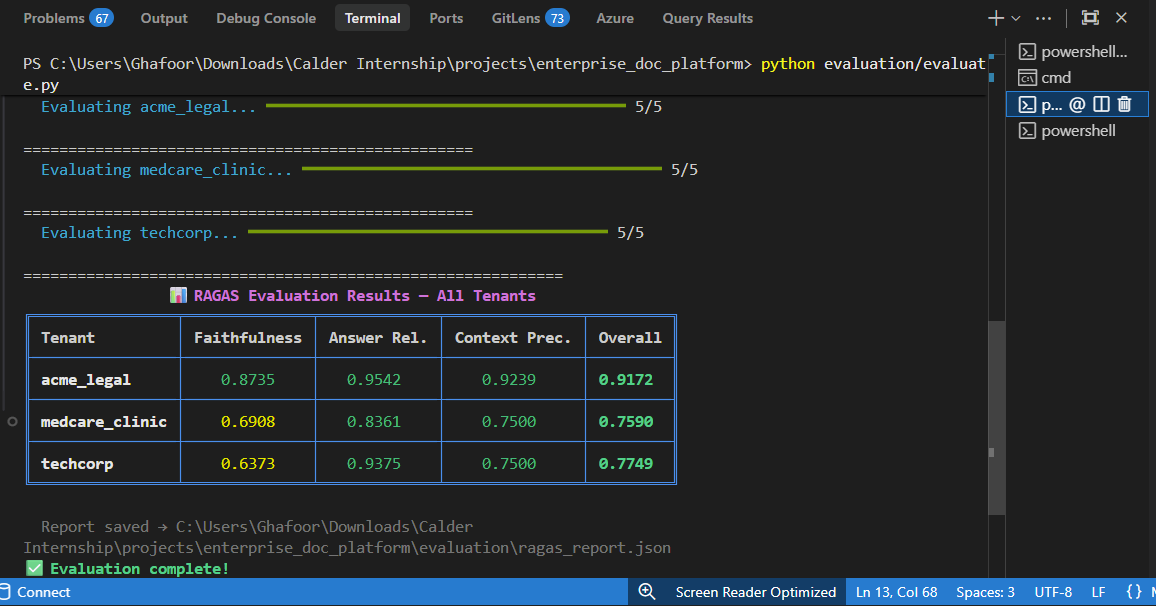
\includegraphics[width=\linewidth, keepaspectratio]{screenshots/Week3/Prod-1.png}
        \caption{FastAPI Multi-Tenant Endpoints}
    \end{minipage}\hfill
    \begin{minipage}{0.48\textwidth}
        \centering
        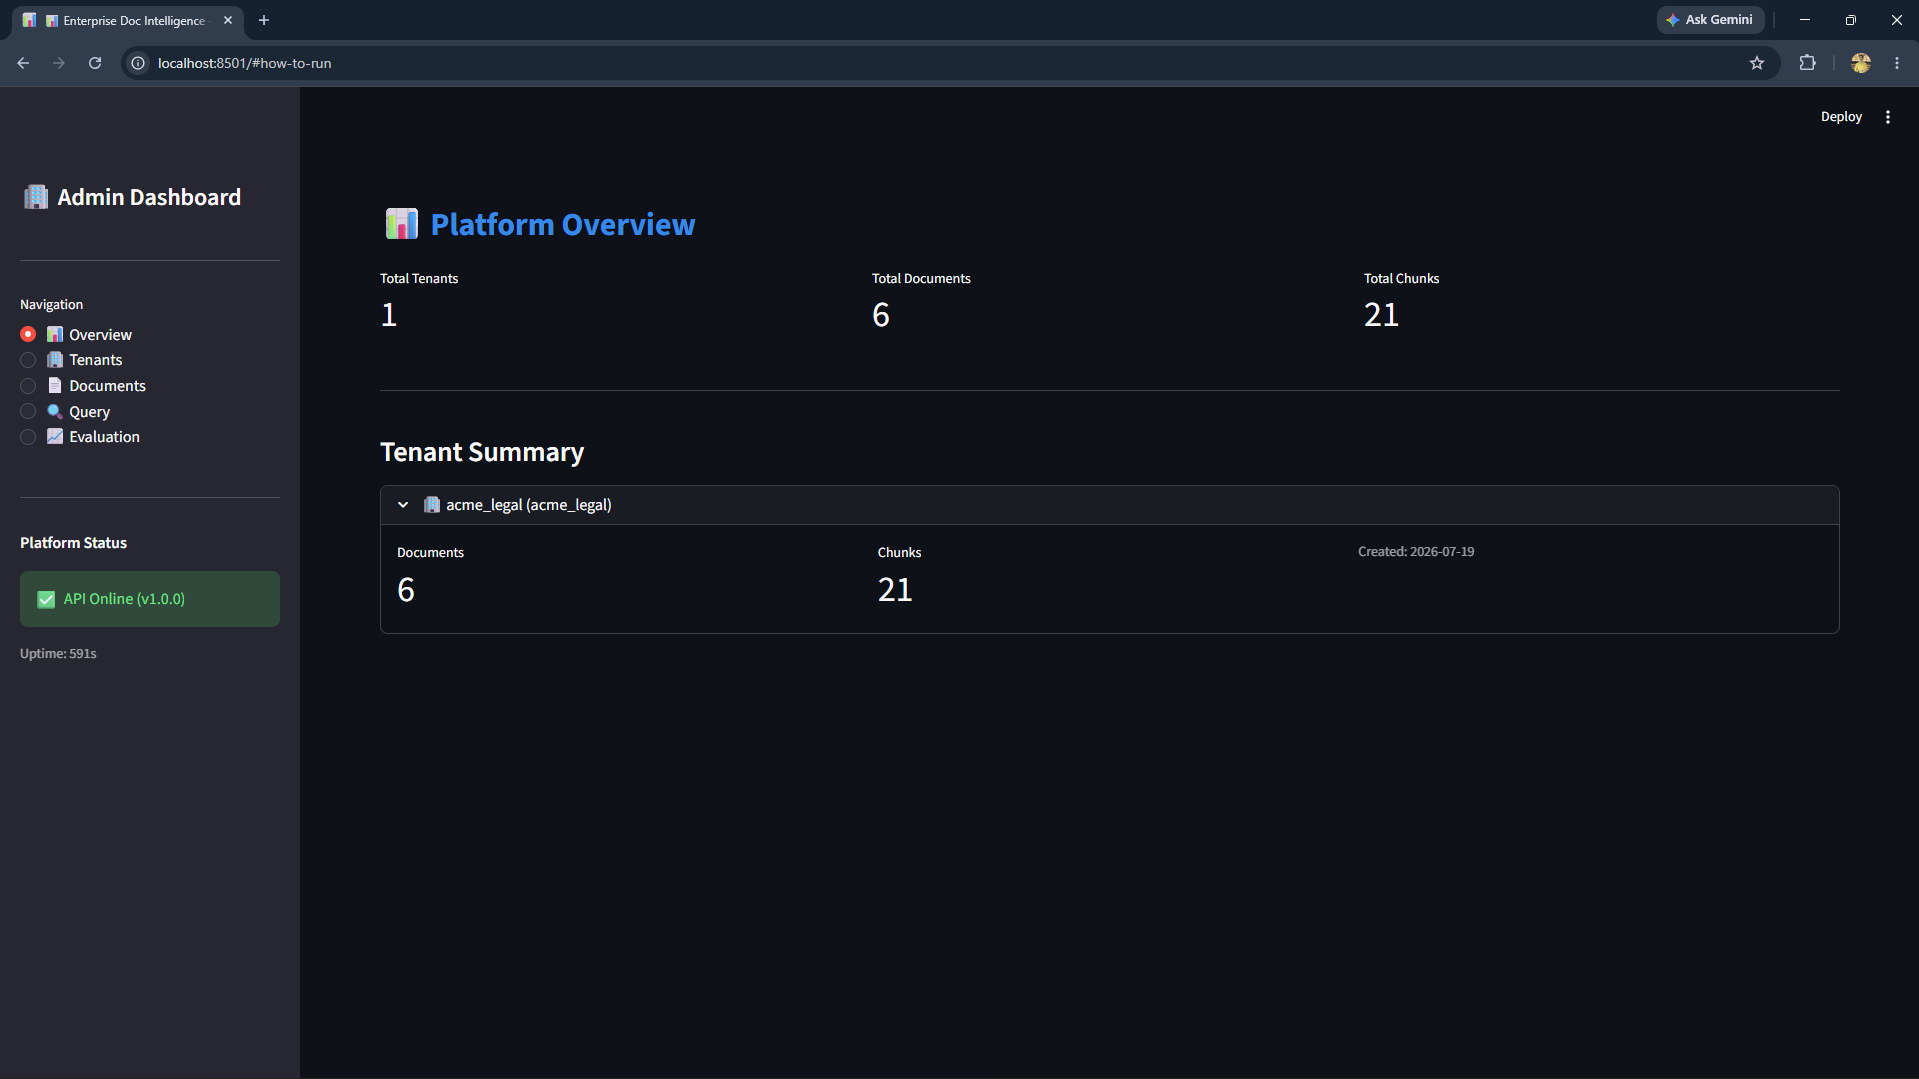
\includegraphics[width=\linewidth, keepaspectratio]{screenshots/Week3/Prod-2.png}
        \caption{Streamlit Admin Dashboard}
    \end{minipage}
\end{figure}

\begin{figure}[H]
    \centering
    \begin{minipage}{0.48\textwidth}
        \centering
        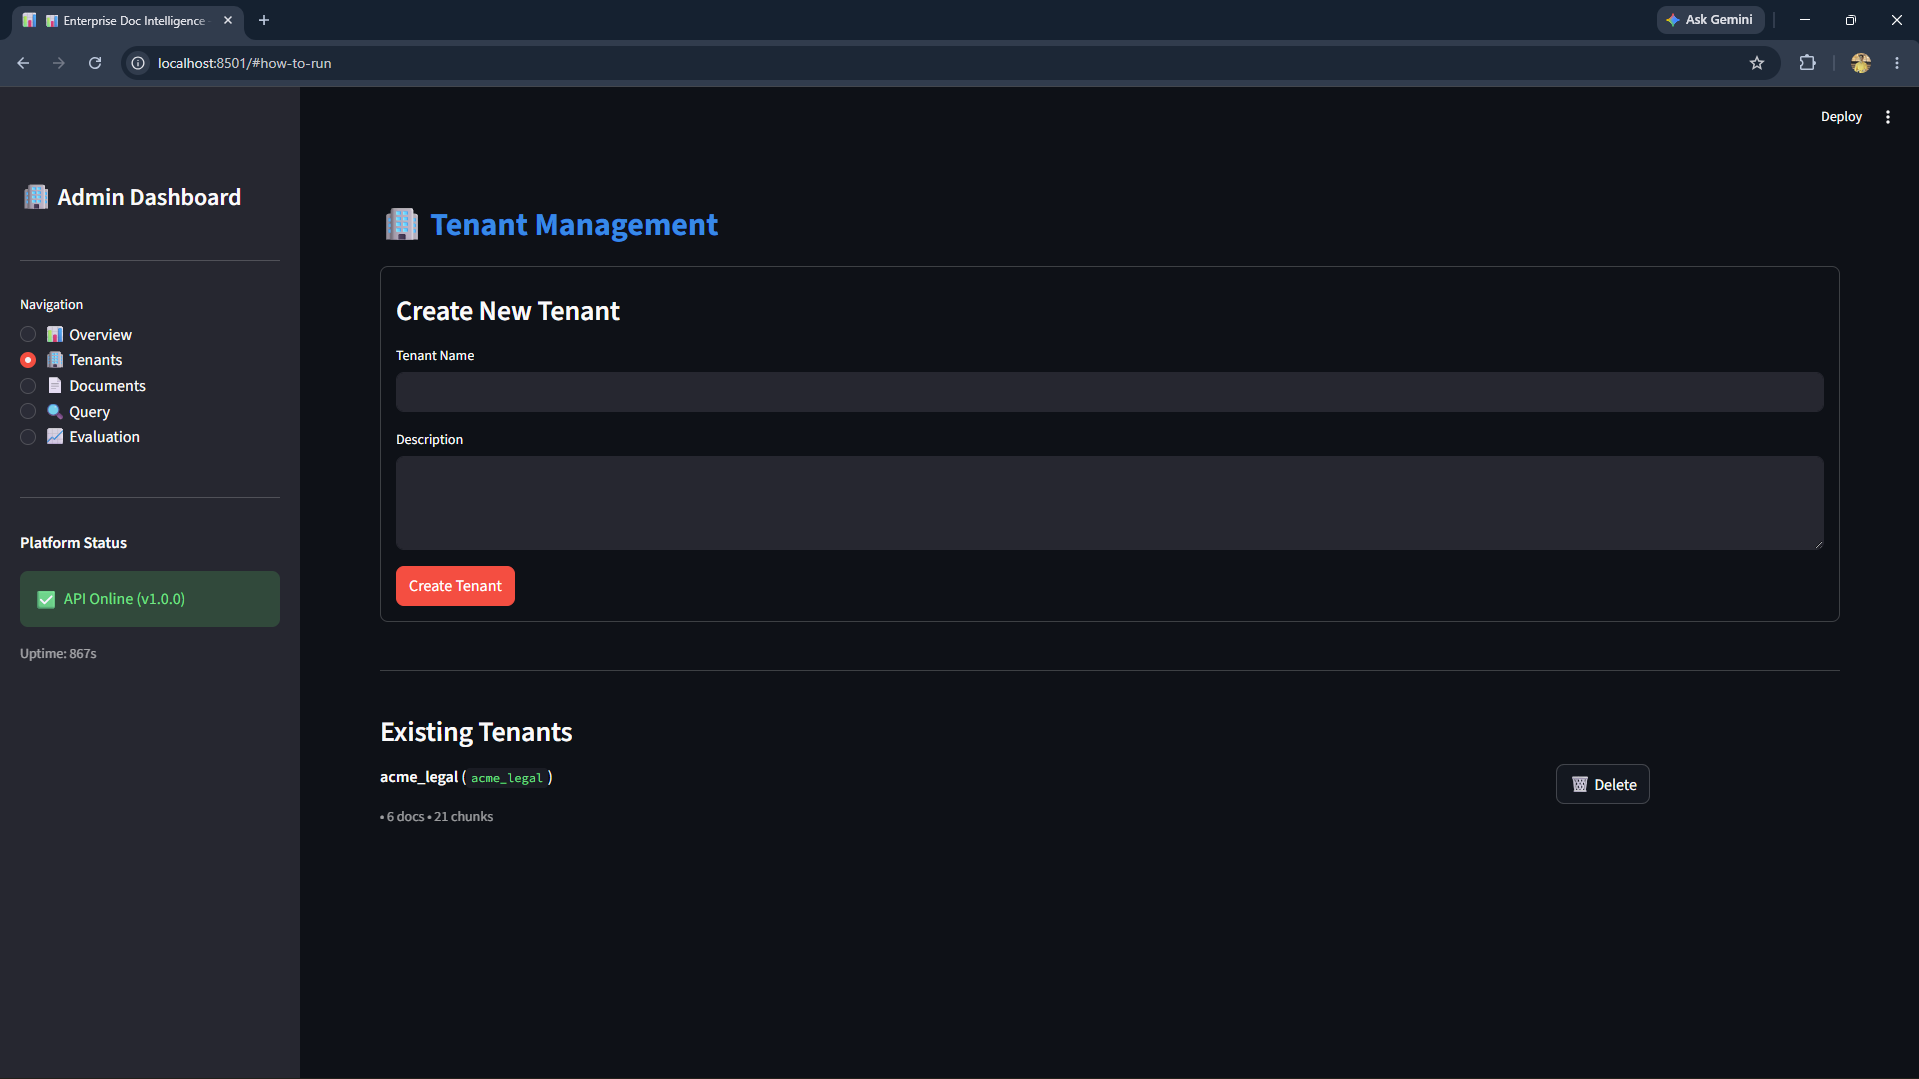
\includegraphics[width=\linewidth, keepaspectratio]{screenshots/Week3/Prod-3.png}
        \caption{Existing Tenants and Management}
    \end{minipage}\hfill
    \begin{minipage}{0.48\textwidth}
        \centering
        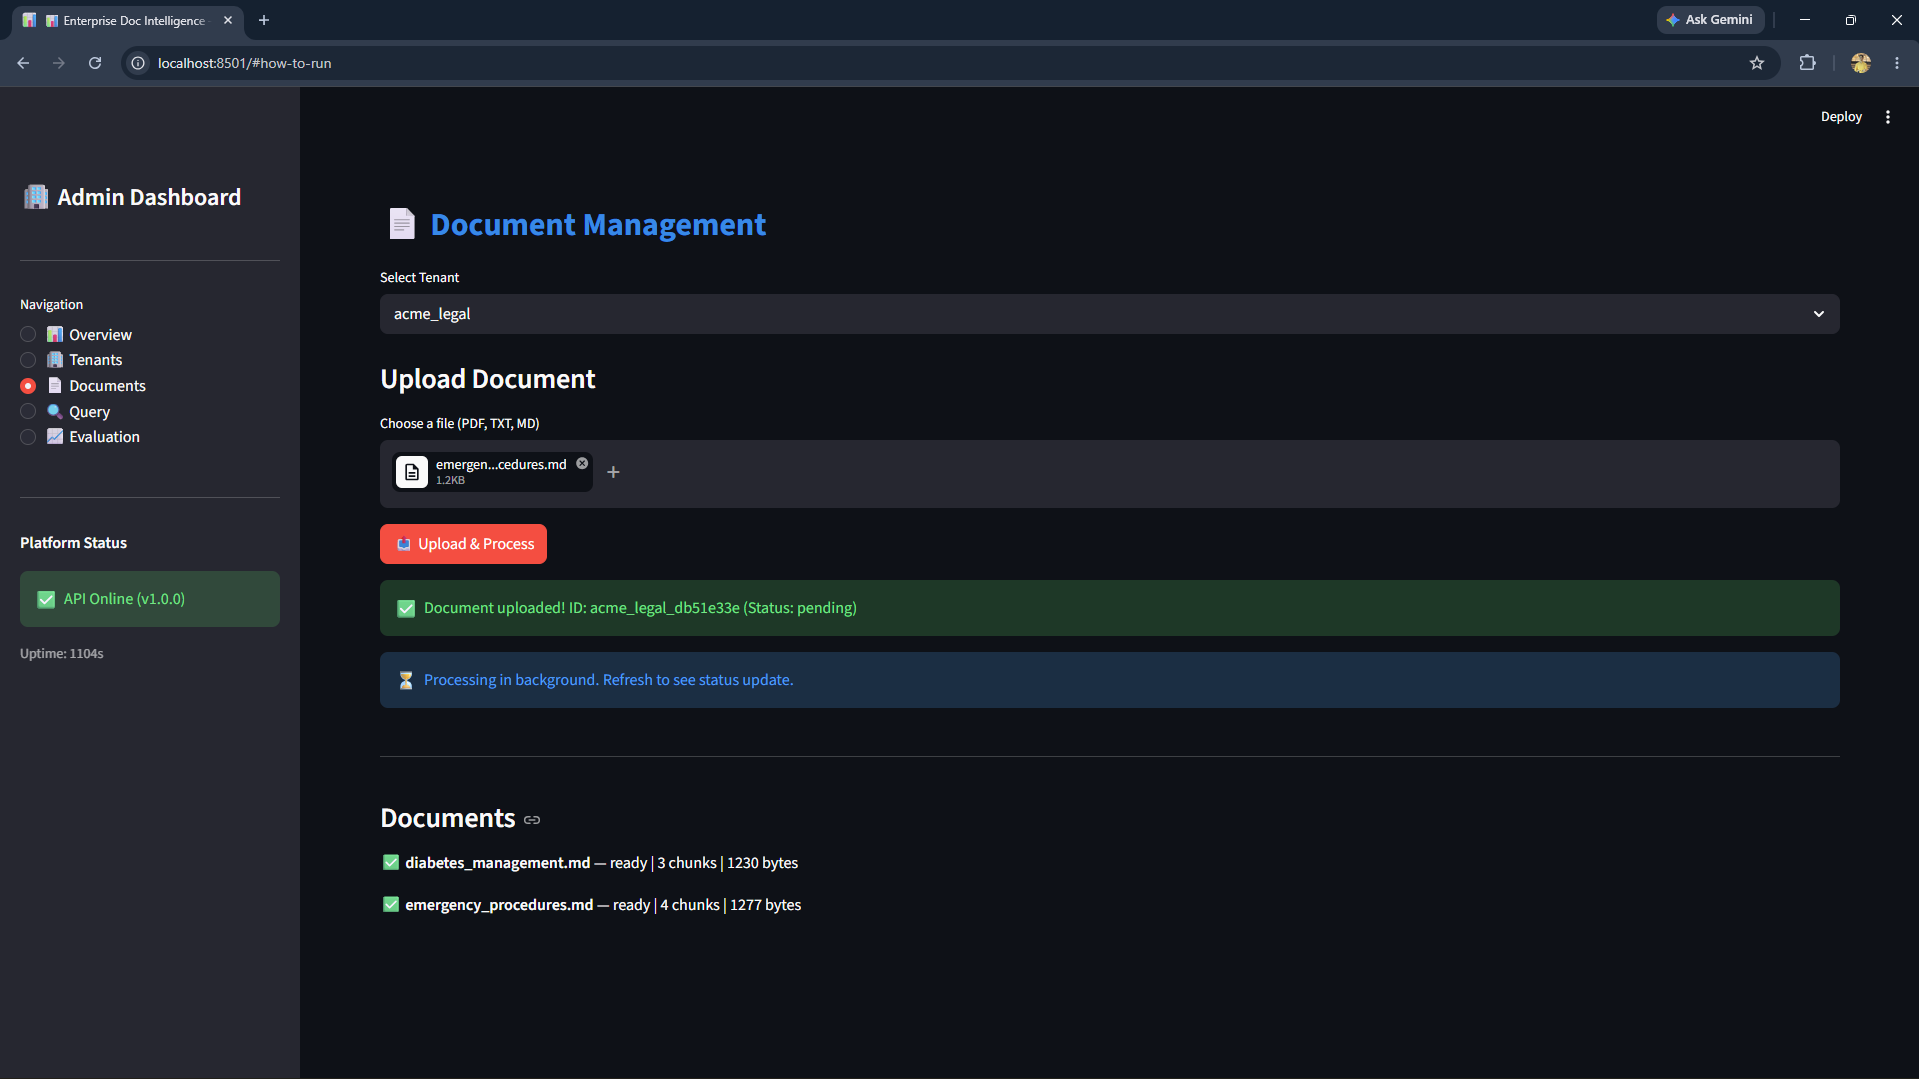
\includegraphics[width=\linewidth, keepaspectratio]{screenshots/Week3/Prod-4.png}
        \caption{Tenant Document Processing Status}
    \end{minipage}
\end{figure}

\begin{figure}[H]
    \centering
    \begin{minipage}{0.48\textwidth}
        \centering
        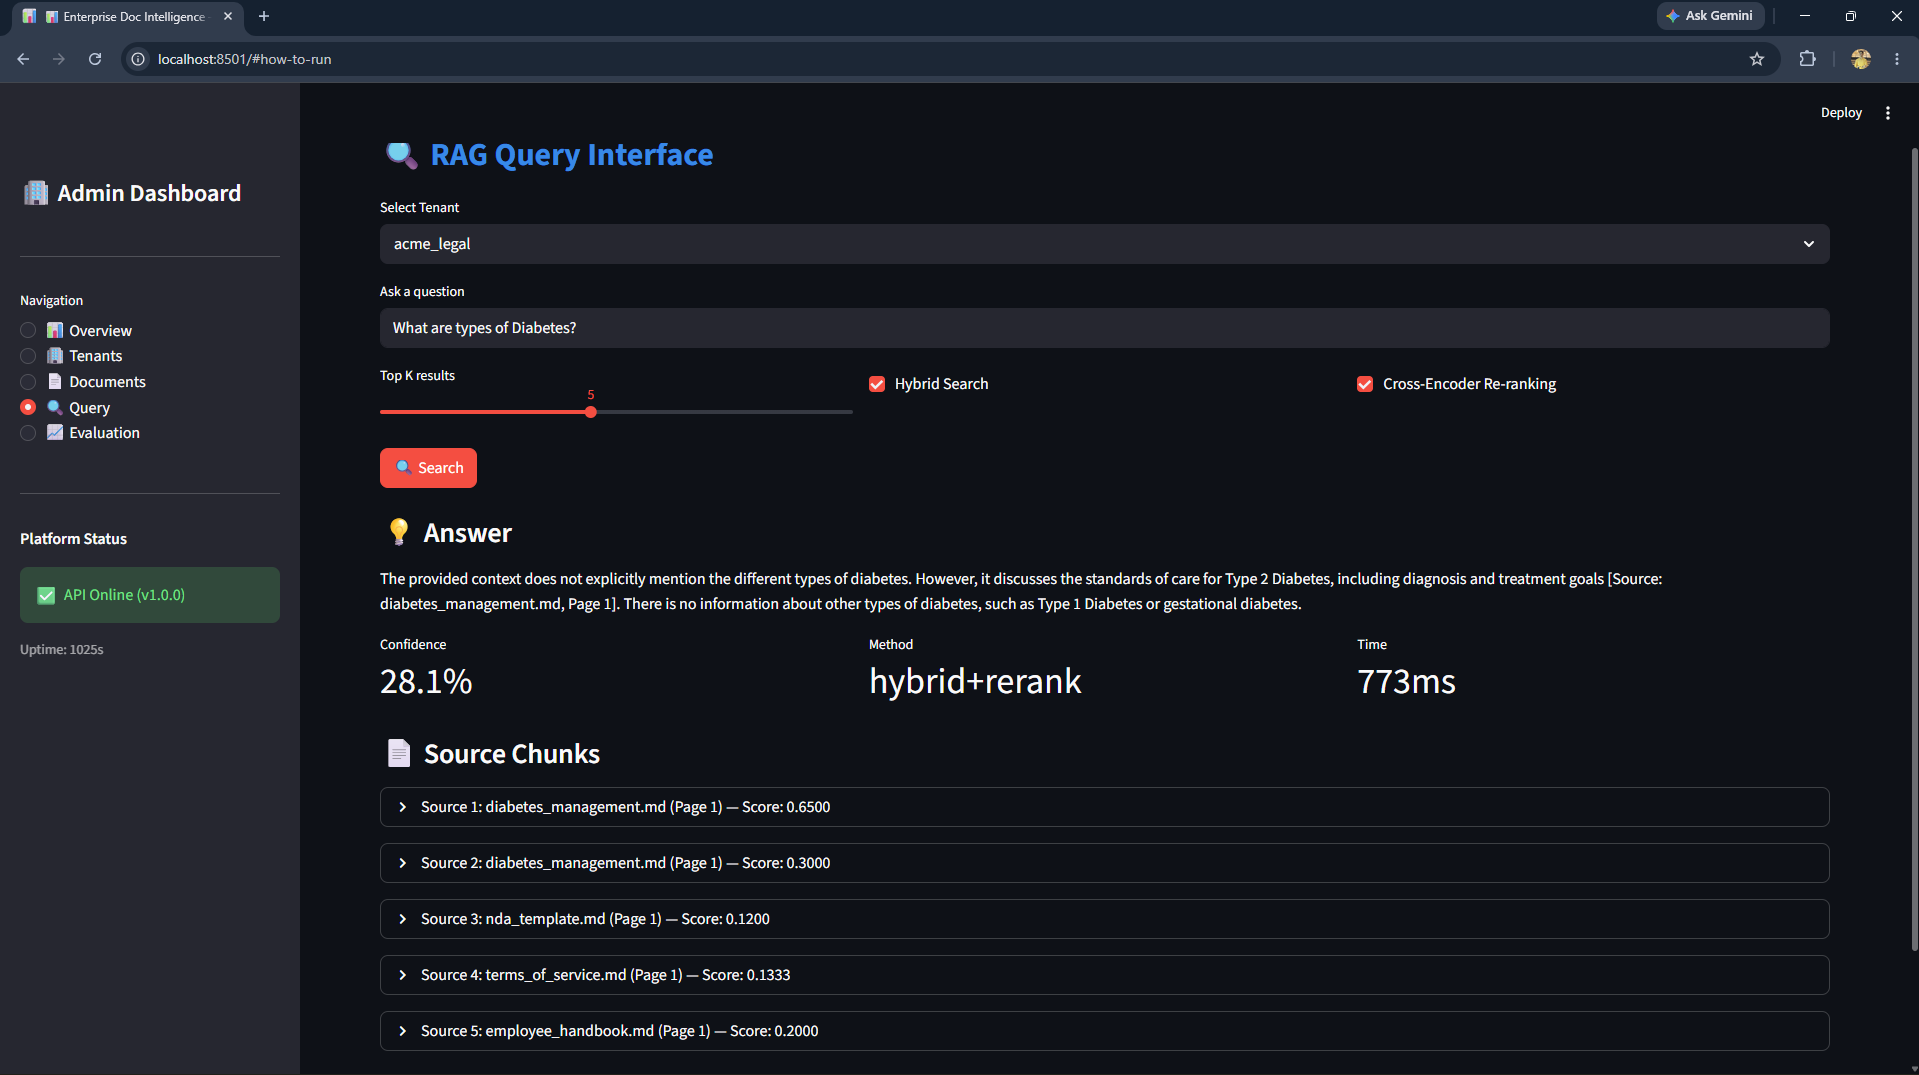
\includegraphics[width=\linewidth, keepaspectratio]{screenshots/Week3/Prod-5.png}
        \caption{Advanced Query Retrieval Results}
    \end{minipage}\hfill
    \begin{minipage}{0.48\textwidth}
        \centering
        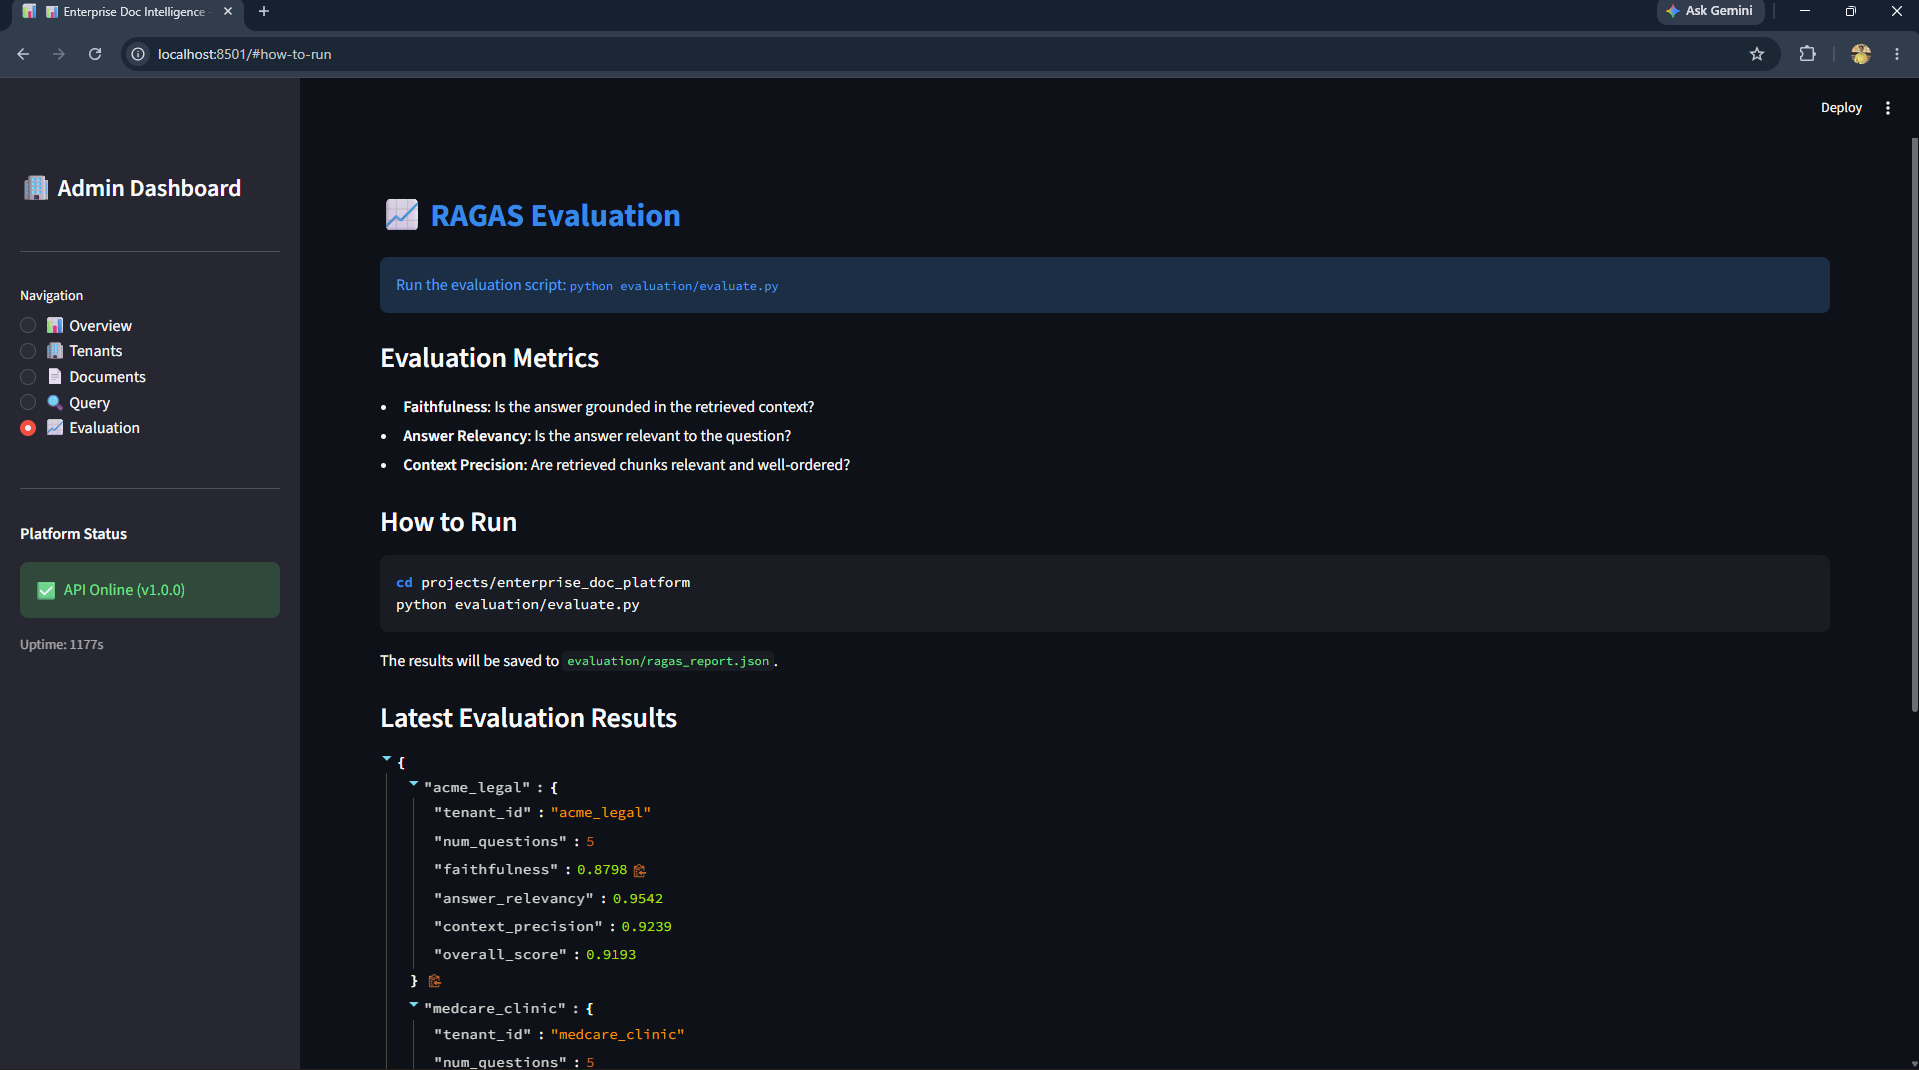
\includegraphics[width=\linewidth, keepaspectratio]{screenshots/Week3/Prod-6.png}
        \caption{RAGAS Evaluation Commands and Guidelines}
    \end{minipage}
\end{figure}

\begin{figure}[H]
    \centering
    \begin{minipage}{0.5\textwidth}
        \centering
        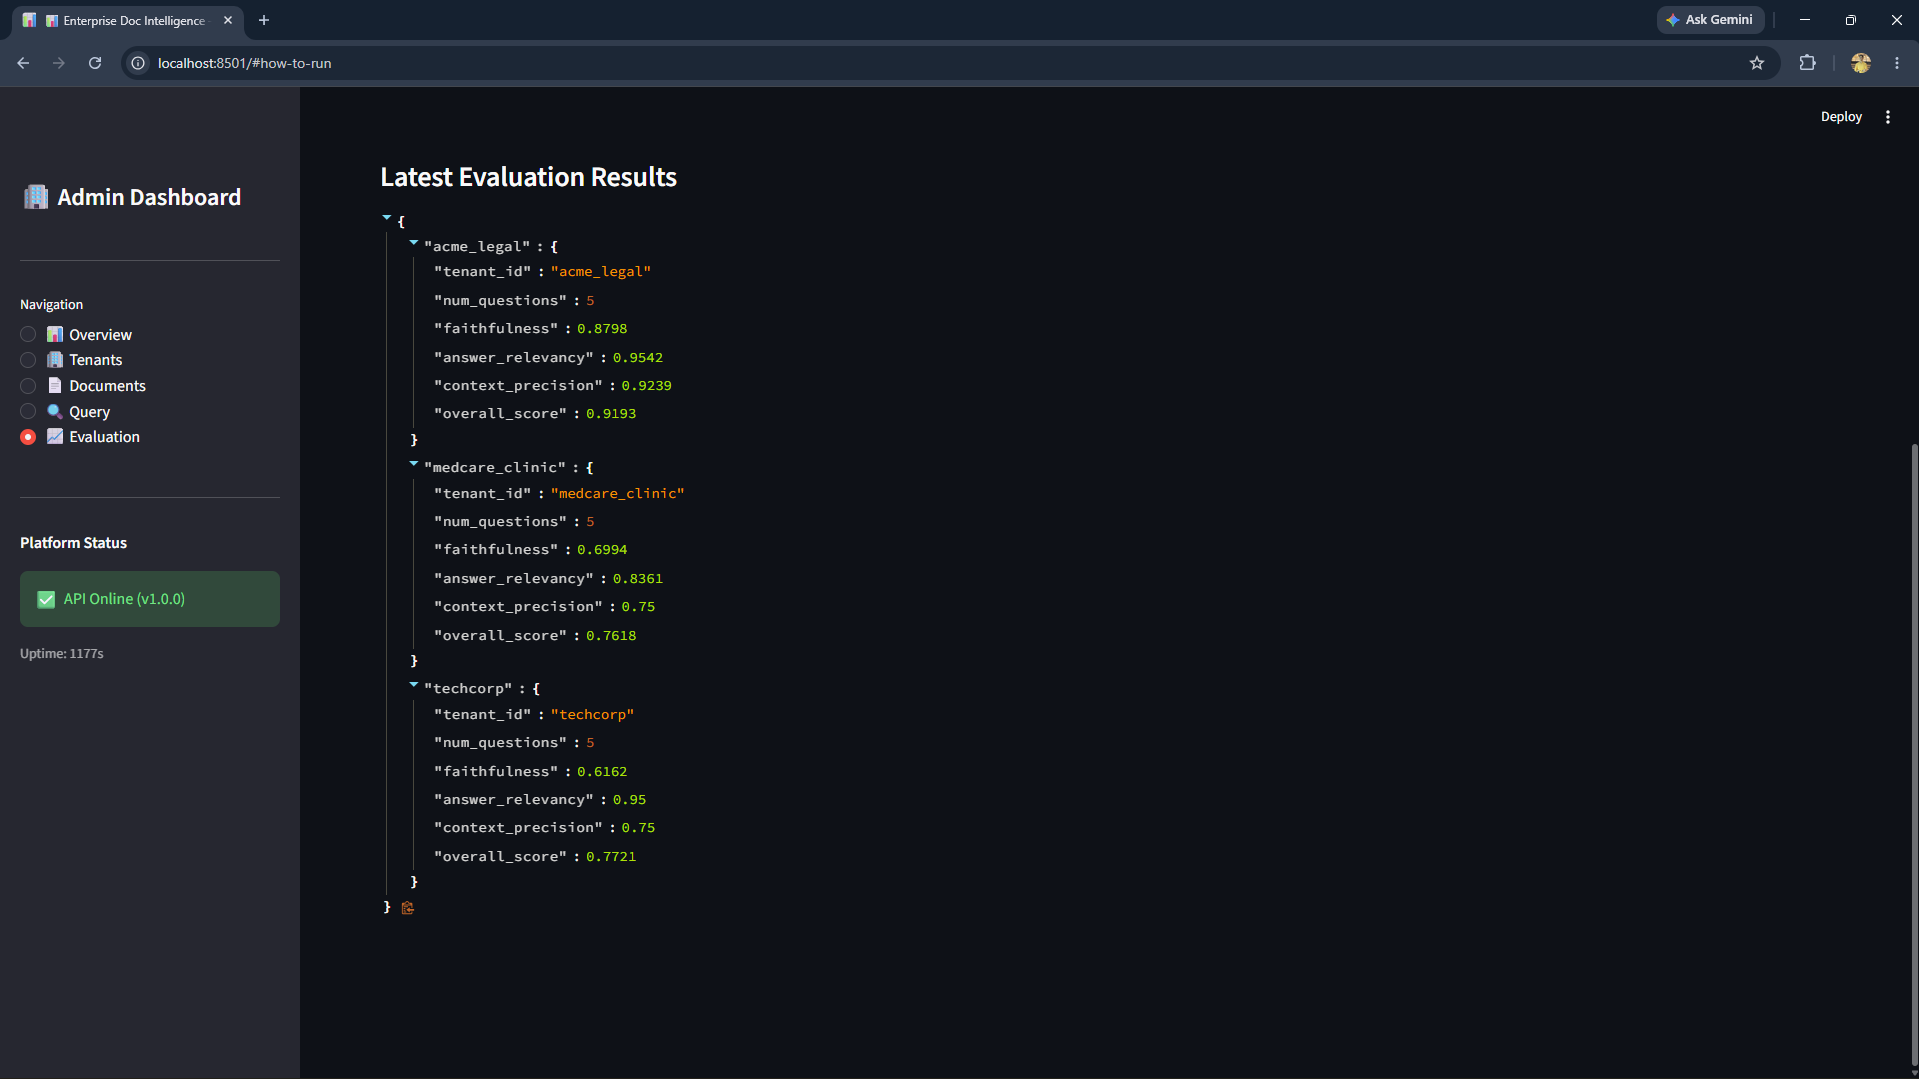
\includegraphics[width=\linewidth, keepaspectratio]{screenshots/Week3/Prod-7.png}
        \caption{RAGAS Evaluation Scores \& Confidence Metrics}
    \end{minipage}
\end{figure}

\newpage

% --- Section 4: Intermediate Project ---
\section{Intermediate Project: Personal Knowledge Base}

\begin{tcolorbox}[colback=accent, colframe=primary, title=\textbf{Architectural Overview}, boxrule=1pt]
A CLI-based multi-document Question and Answer system. This agent ingests disparate file formats (PDFs, text files, markdown), chunks the text, and stores the embeddings in a local ChromaDB instance, allowing the user to dynamically query their own customized, local knowledge repository.
\end{tcolorbox}

\subsection{Technical Implementation}
\begin{itemize}[label=\textcolor{secondary}{$\bullet$}]
    \item \textbf{Multi-Format Document Loaders:} Utilized LangChain loaders to seamlessly ingest structured and unstructured data formats.
    \item \textbf{Chunking \& Local Embeddings:} Experimented with RecursiveCharacterTextSplitter and embedded the resulting chunks utilizing local \texttt{sentence-transformers} to avoid third-party API costs.
    \item \textbf{LangChain RetrievalQA:} Orchestrated the retrieval and generation phases using LangChain's modular chains, ensuring every generated answer is heavily grounded by citing specific document chunks and metadata.
\end{itemize}

\subsection{System Demonstrations}
\begin{figure}[H]
    \centering
    \begin{minipage}{0.48\textwidth}
        \centering
        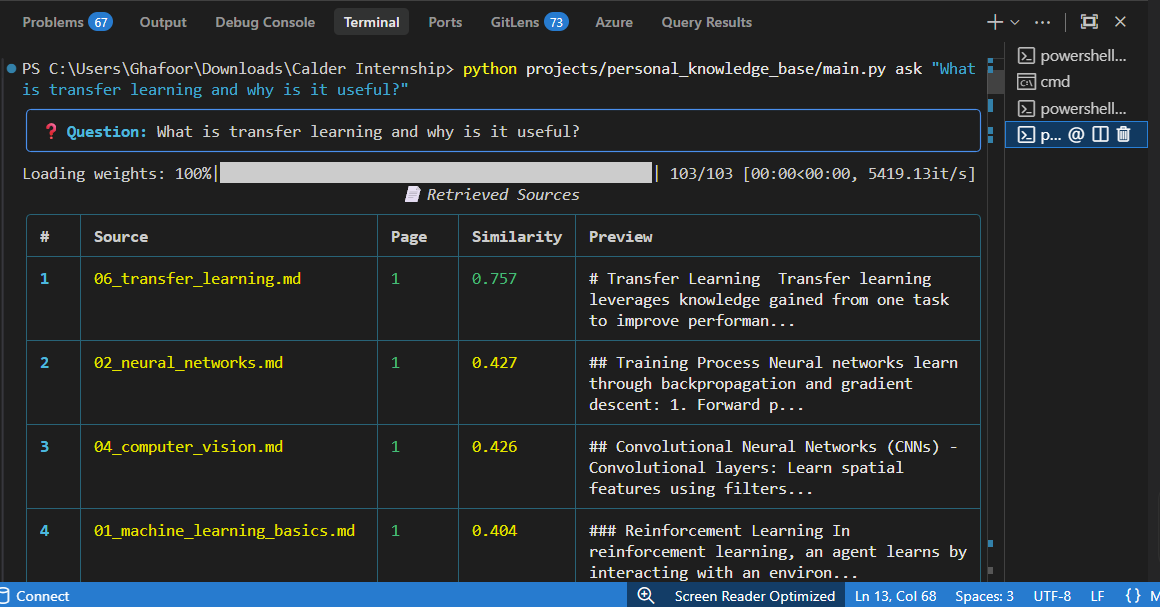
\includegraphics[width=\linewidth, keepaspectratio]{screenshots/Week3/Inter-1.png}
        \caption{CLI Initialization \& Database Setup}
    \end{minipage}\hfill
    \begin{minipage}{0.48\textwidth}
        \centering
        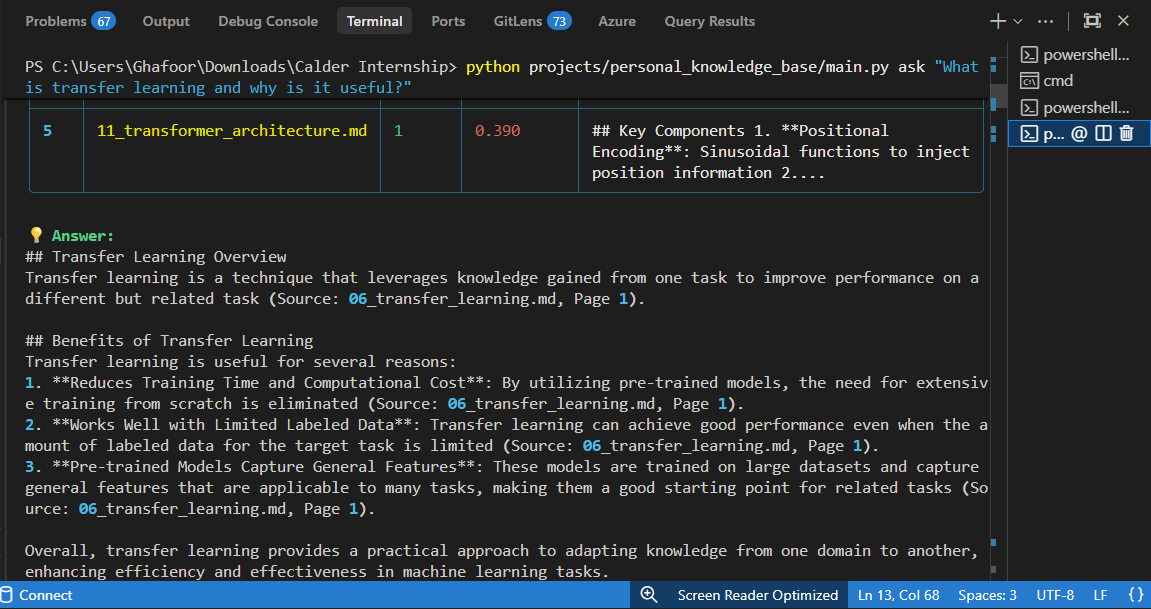
\includegraphics[width=\linewidth, keepaspectratio]{screenshots/Week3/Inter-2.png}
        \caption{Document Parsing and Chunking}
    \end{minipage}
\end{figure}

\vspace{0.3cm}

\begin{figure}[H]
    \centering
    \begin{minipage}{0.48\textwidth}
        \centering
        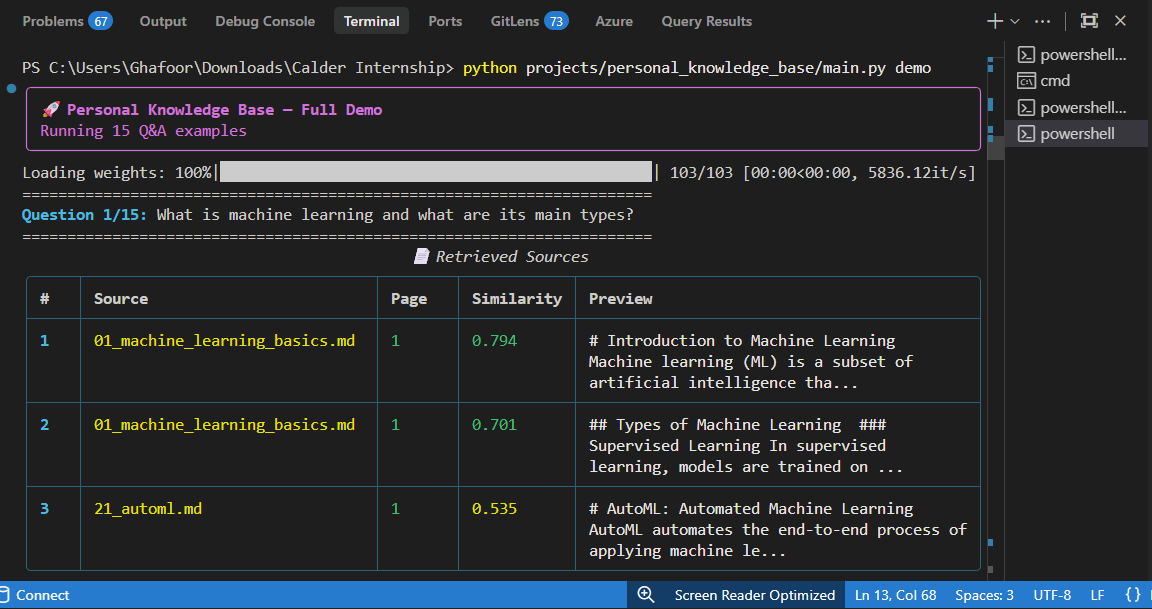
\includegraphics[width=\linewidth, keepaspectratio]{screenshots/Week3/Inter-3.png}
        \caption{ChromaDB Vector Ingestion}
    \end{minipage}\hfill
    \begin{minipage}{0.48\textwidth}
        \centering
        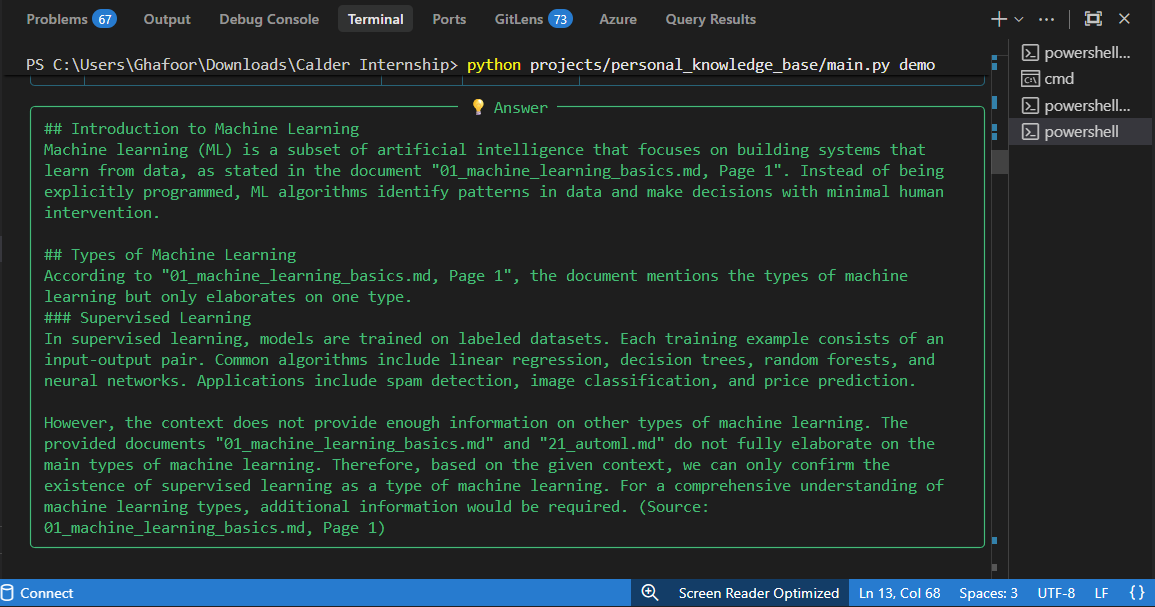
\includegraphics[width=\linewidth, keepaspectratio]{screenshots/Week3/Inter-4.png}
        \caption{Querying the Local Knowledge Base}
    \end{minipage}
\end{figure}

\begin{figure}[H]
    \centering
    \begin{minipage}{0.48\textwidth}
        \centering
        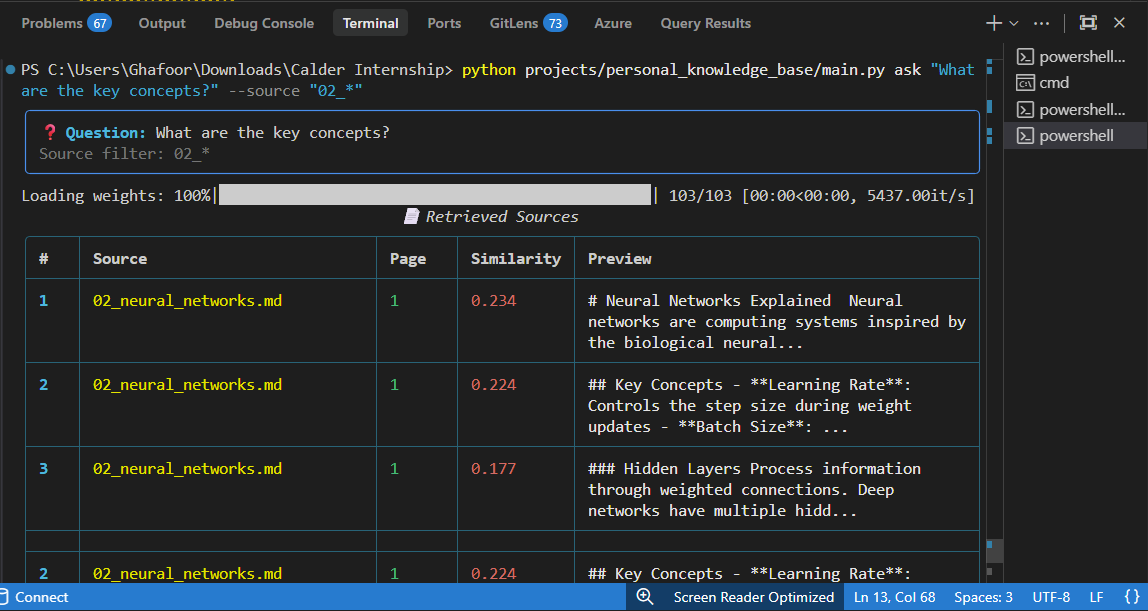
\includegraphics[width=\linewidth, keepaspectratio]{screenshots/Week3/Inter-5.png}
        \caption{Response Generation \& Source Sourcing}
    \end{minipage}\hfill
    \begin{minipage}{0.48\textwidth}
        \centering
        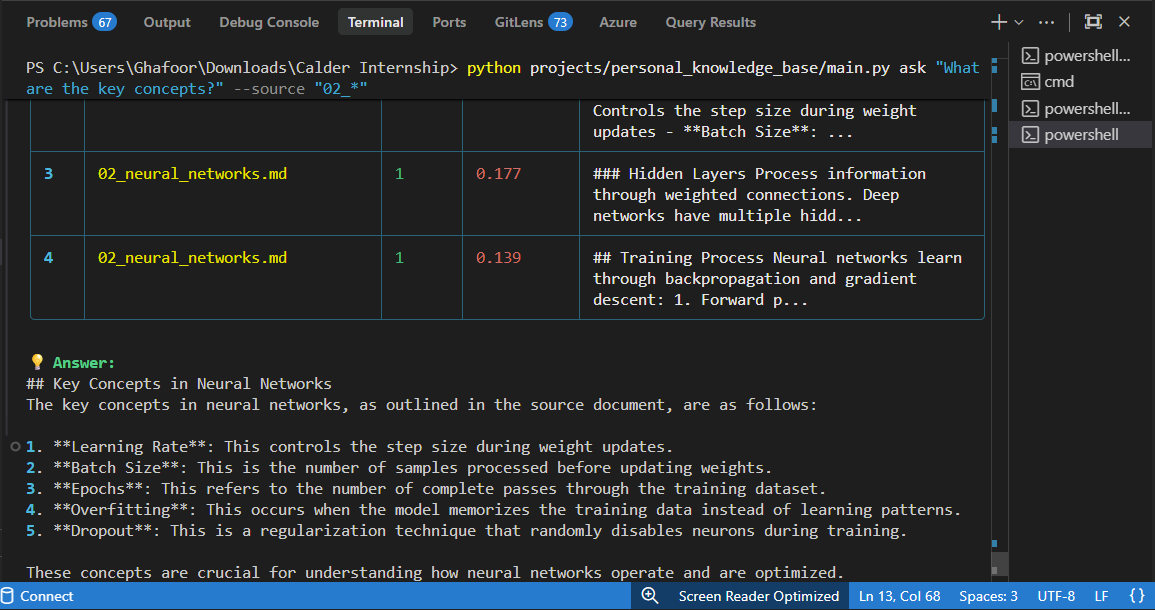
\includegraphics[width=\linewidth, keepaspectratio]{screenshots/Week3/Inter-6.png}
        \caption{Streaming Responses in the CLI}
    \end{minipage}
\end{figure}

\newpage

% --- Section 5: Foundational Labs ---
\section{Foundational Labs Deep-Dive}

\subsection{Lab 3.1: Semantic Search CLI}
Focused on the core mathematics of vector similarity and local embedding models.
\begin{itemize}[label=\textcolor{secondary}{$\bullet$}]
    \item \textbf{Embedding Spaces:} Computed semantic similarities using Cosine Distance across 100 Wikipedia sentences.
    \item \textbf{Model Comparisons:} Embedded the dataset using two different HuggingFace models (\texttt{all-MiniLM-L6-v2} vs \texttt{bge-small-en}) and visualized the distribution of vectors using 2D PCA.
\end{itemize}

\begin{figure}[H]
    \centering
    \begin{minipage}{0.48\textwidth}
        \centering
        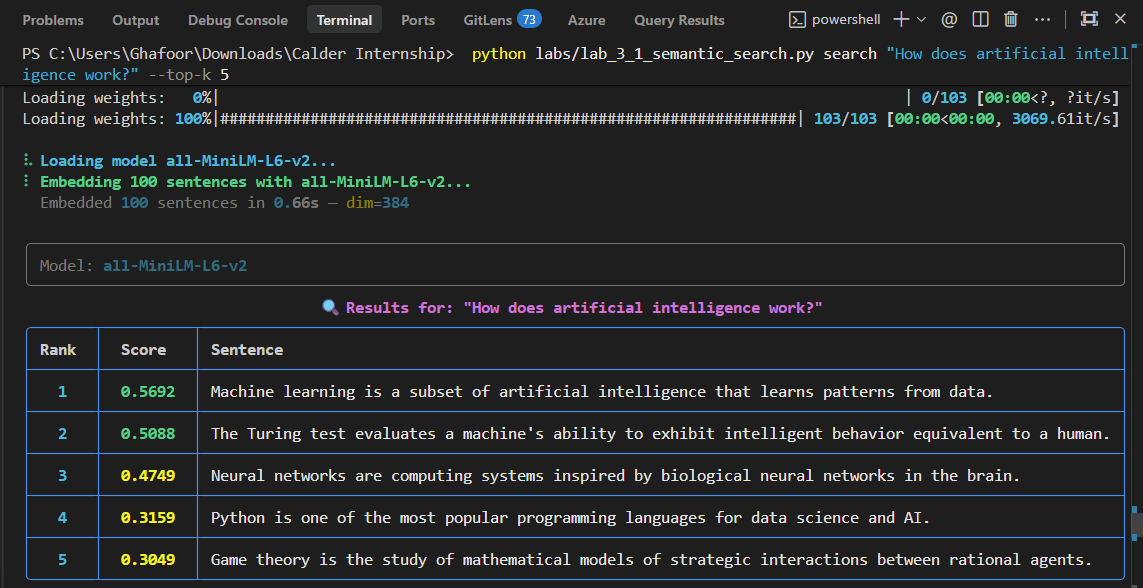
\includegraphics[width=\linewidth]{screenshots/Week3/Lab-3.1-1.png}
        \caption{Sentence Embedding Computations}
    \end{minipage}\hfill
    \begin{minipage}{0.48\textwidth}
        \centering
        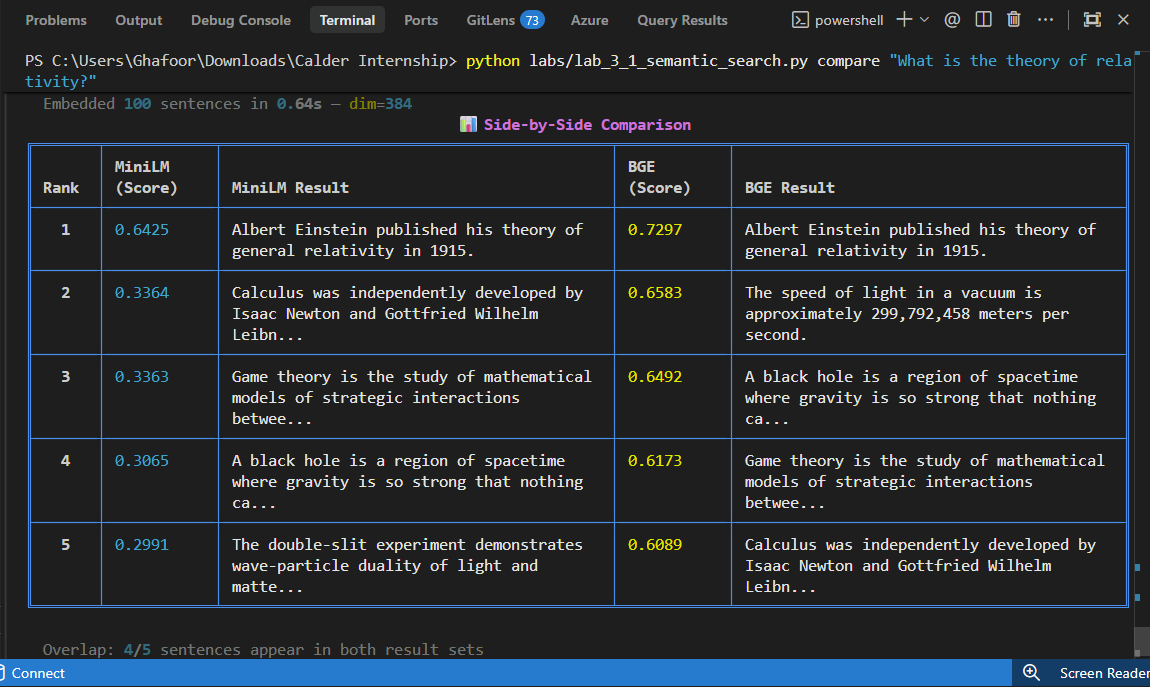
\includegraphics[width=\linewidth]{screenshots/Week3/Lab-3.1-2.png}
        \caption{Cosine Similarity Comparisons}
    \end{minipage}
\end{figure}

\begin{figure}[H]
    \centering
    \begin{minipage}{0.48\textwidth}
        \centering
        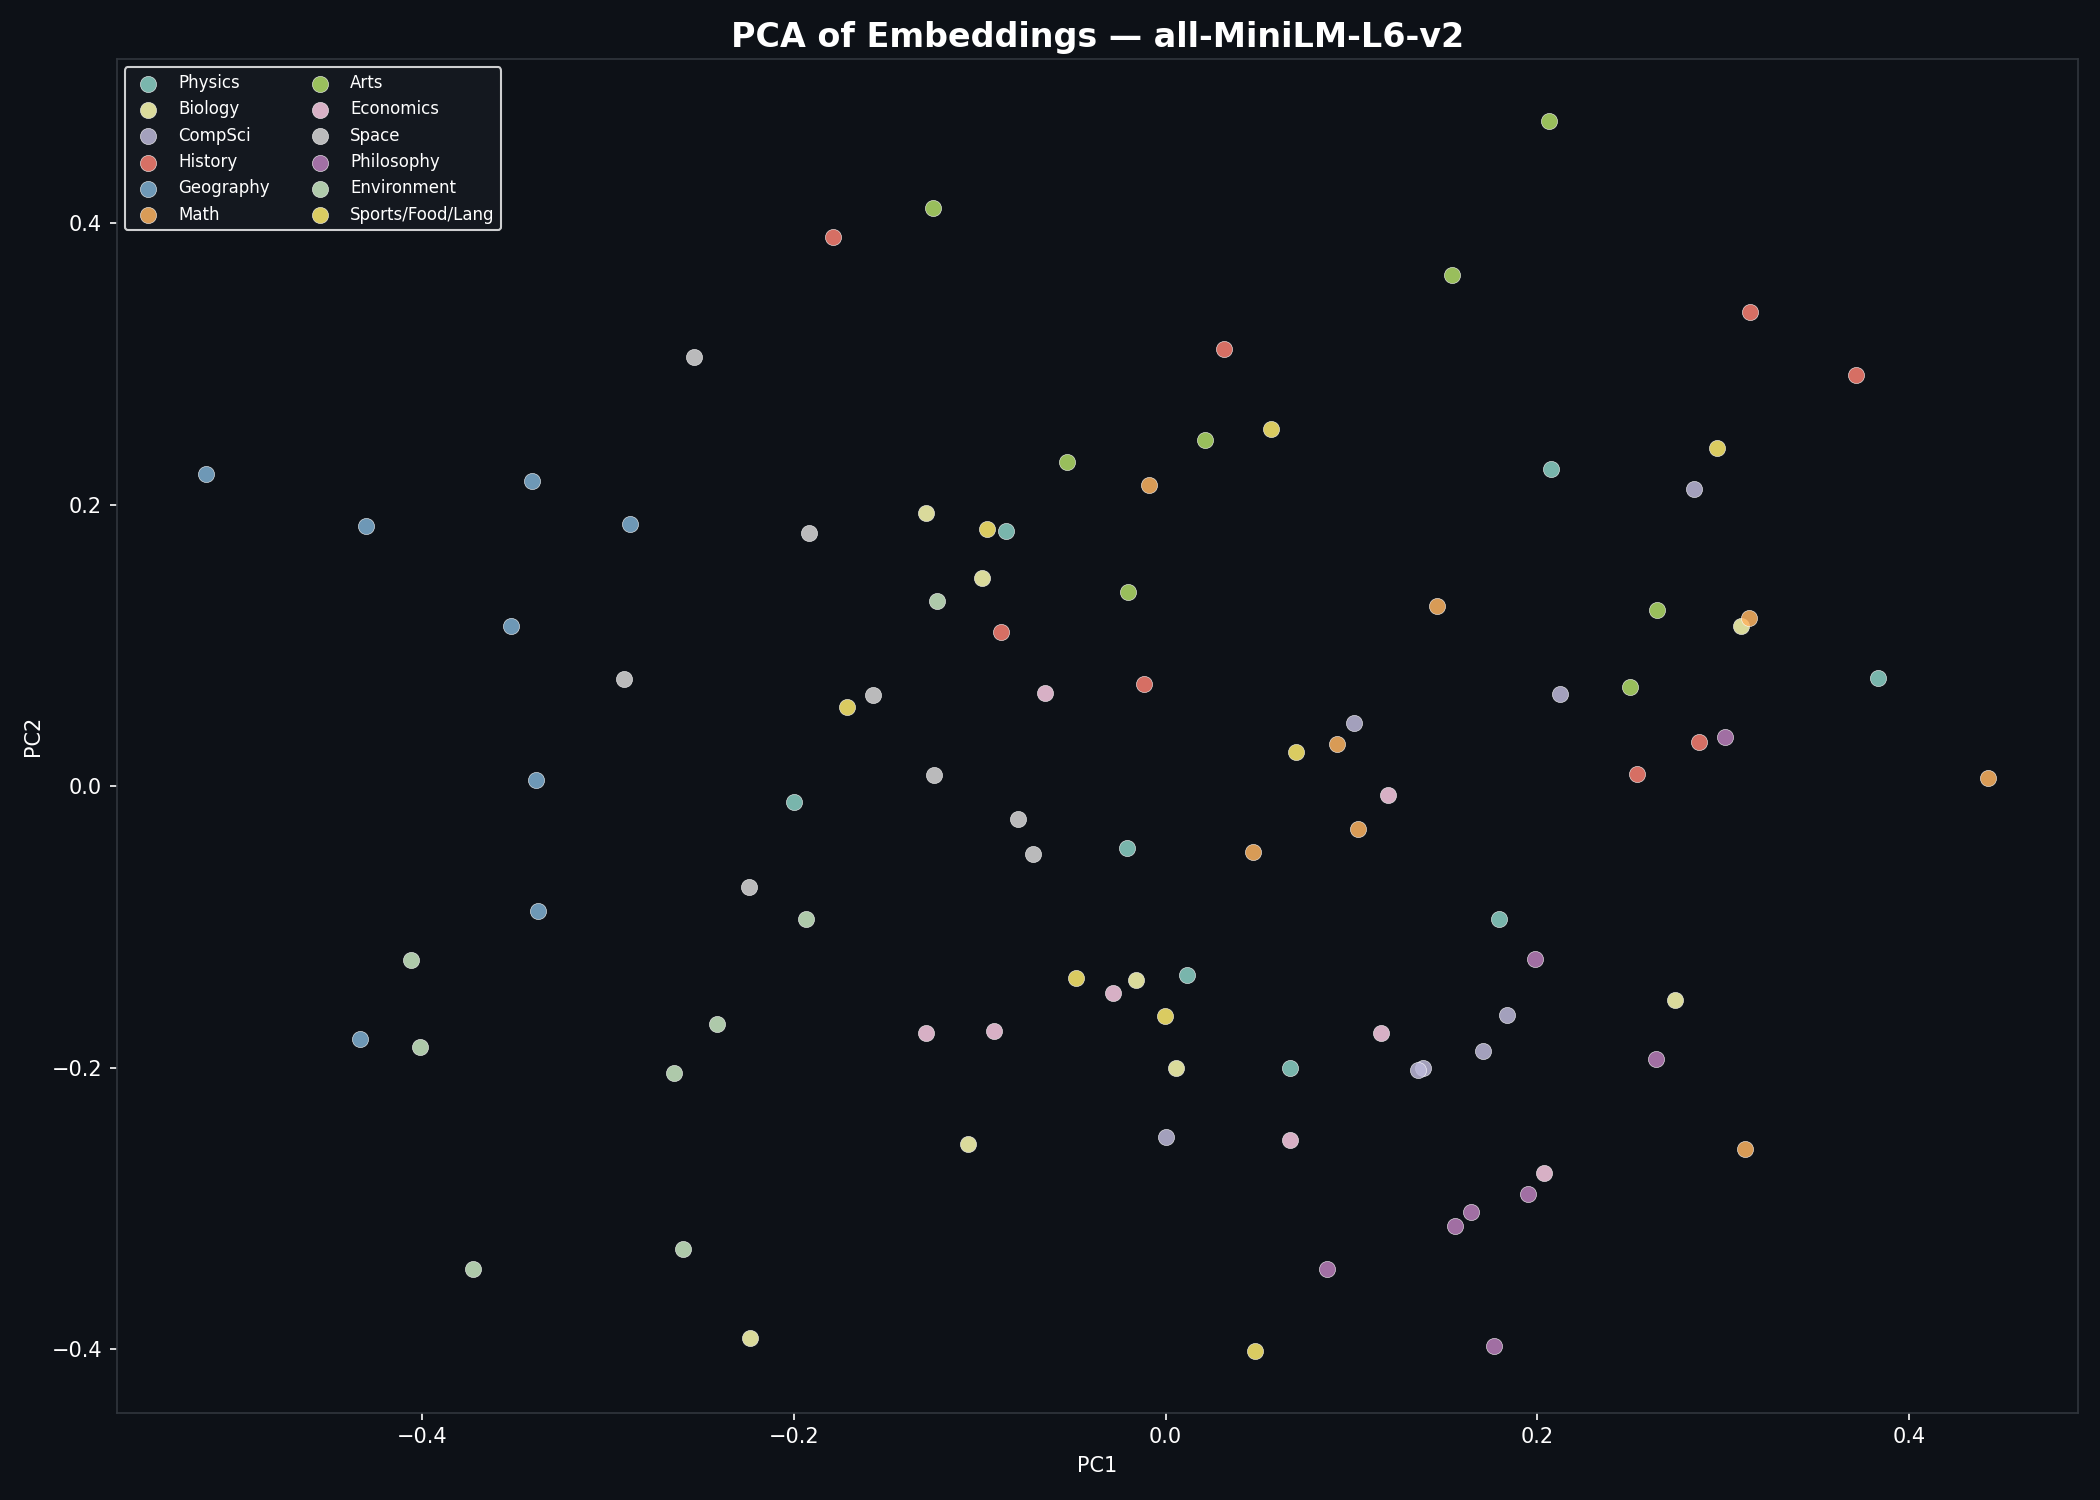
\includegraphics[width=\linewidth]{screenshots/Week3/Lab-3.1-3.png}
        \caption{Model 1 Vector Search Results}
    \end{minipage}\hfill
    \begin{minipage}{0.48\textwidth}
        \centering
        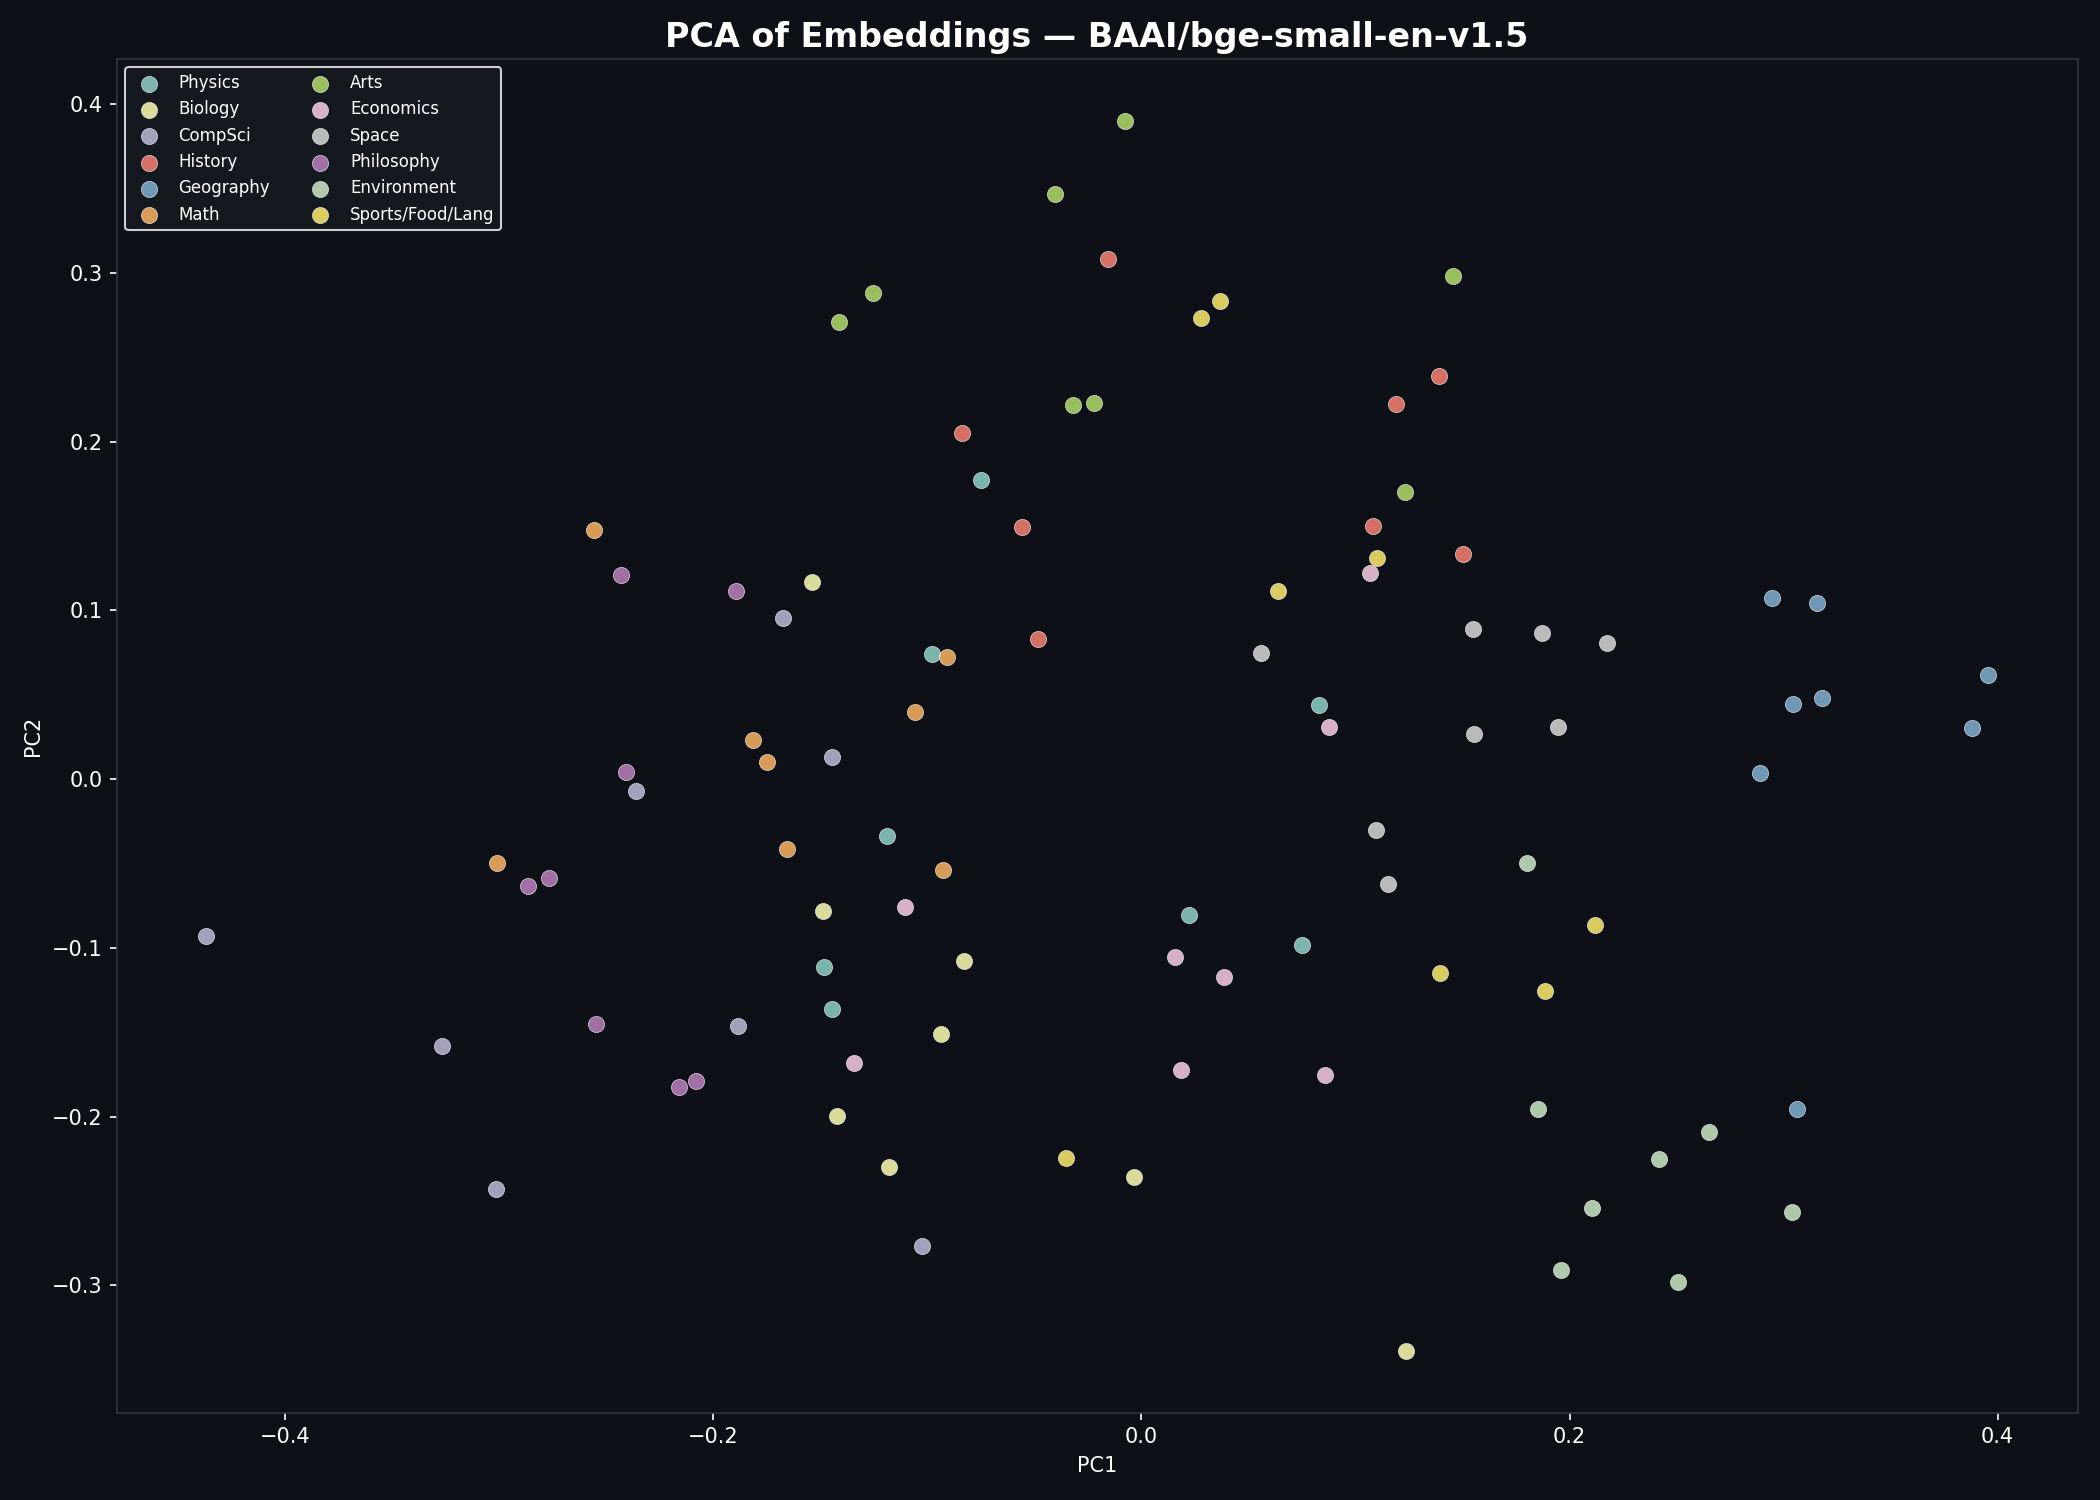
\includegraphics[width=\linewidth]{screenshots/Week3/Lab-3.1-4.png}
        \caption{Model 2 Vector Search Results}
    \end{minipage}
\end{figure}

\begin{figure}[H]
    \centering
    \begin{minipage}{0.5\textwidth}
        \centering
        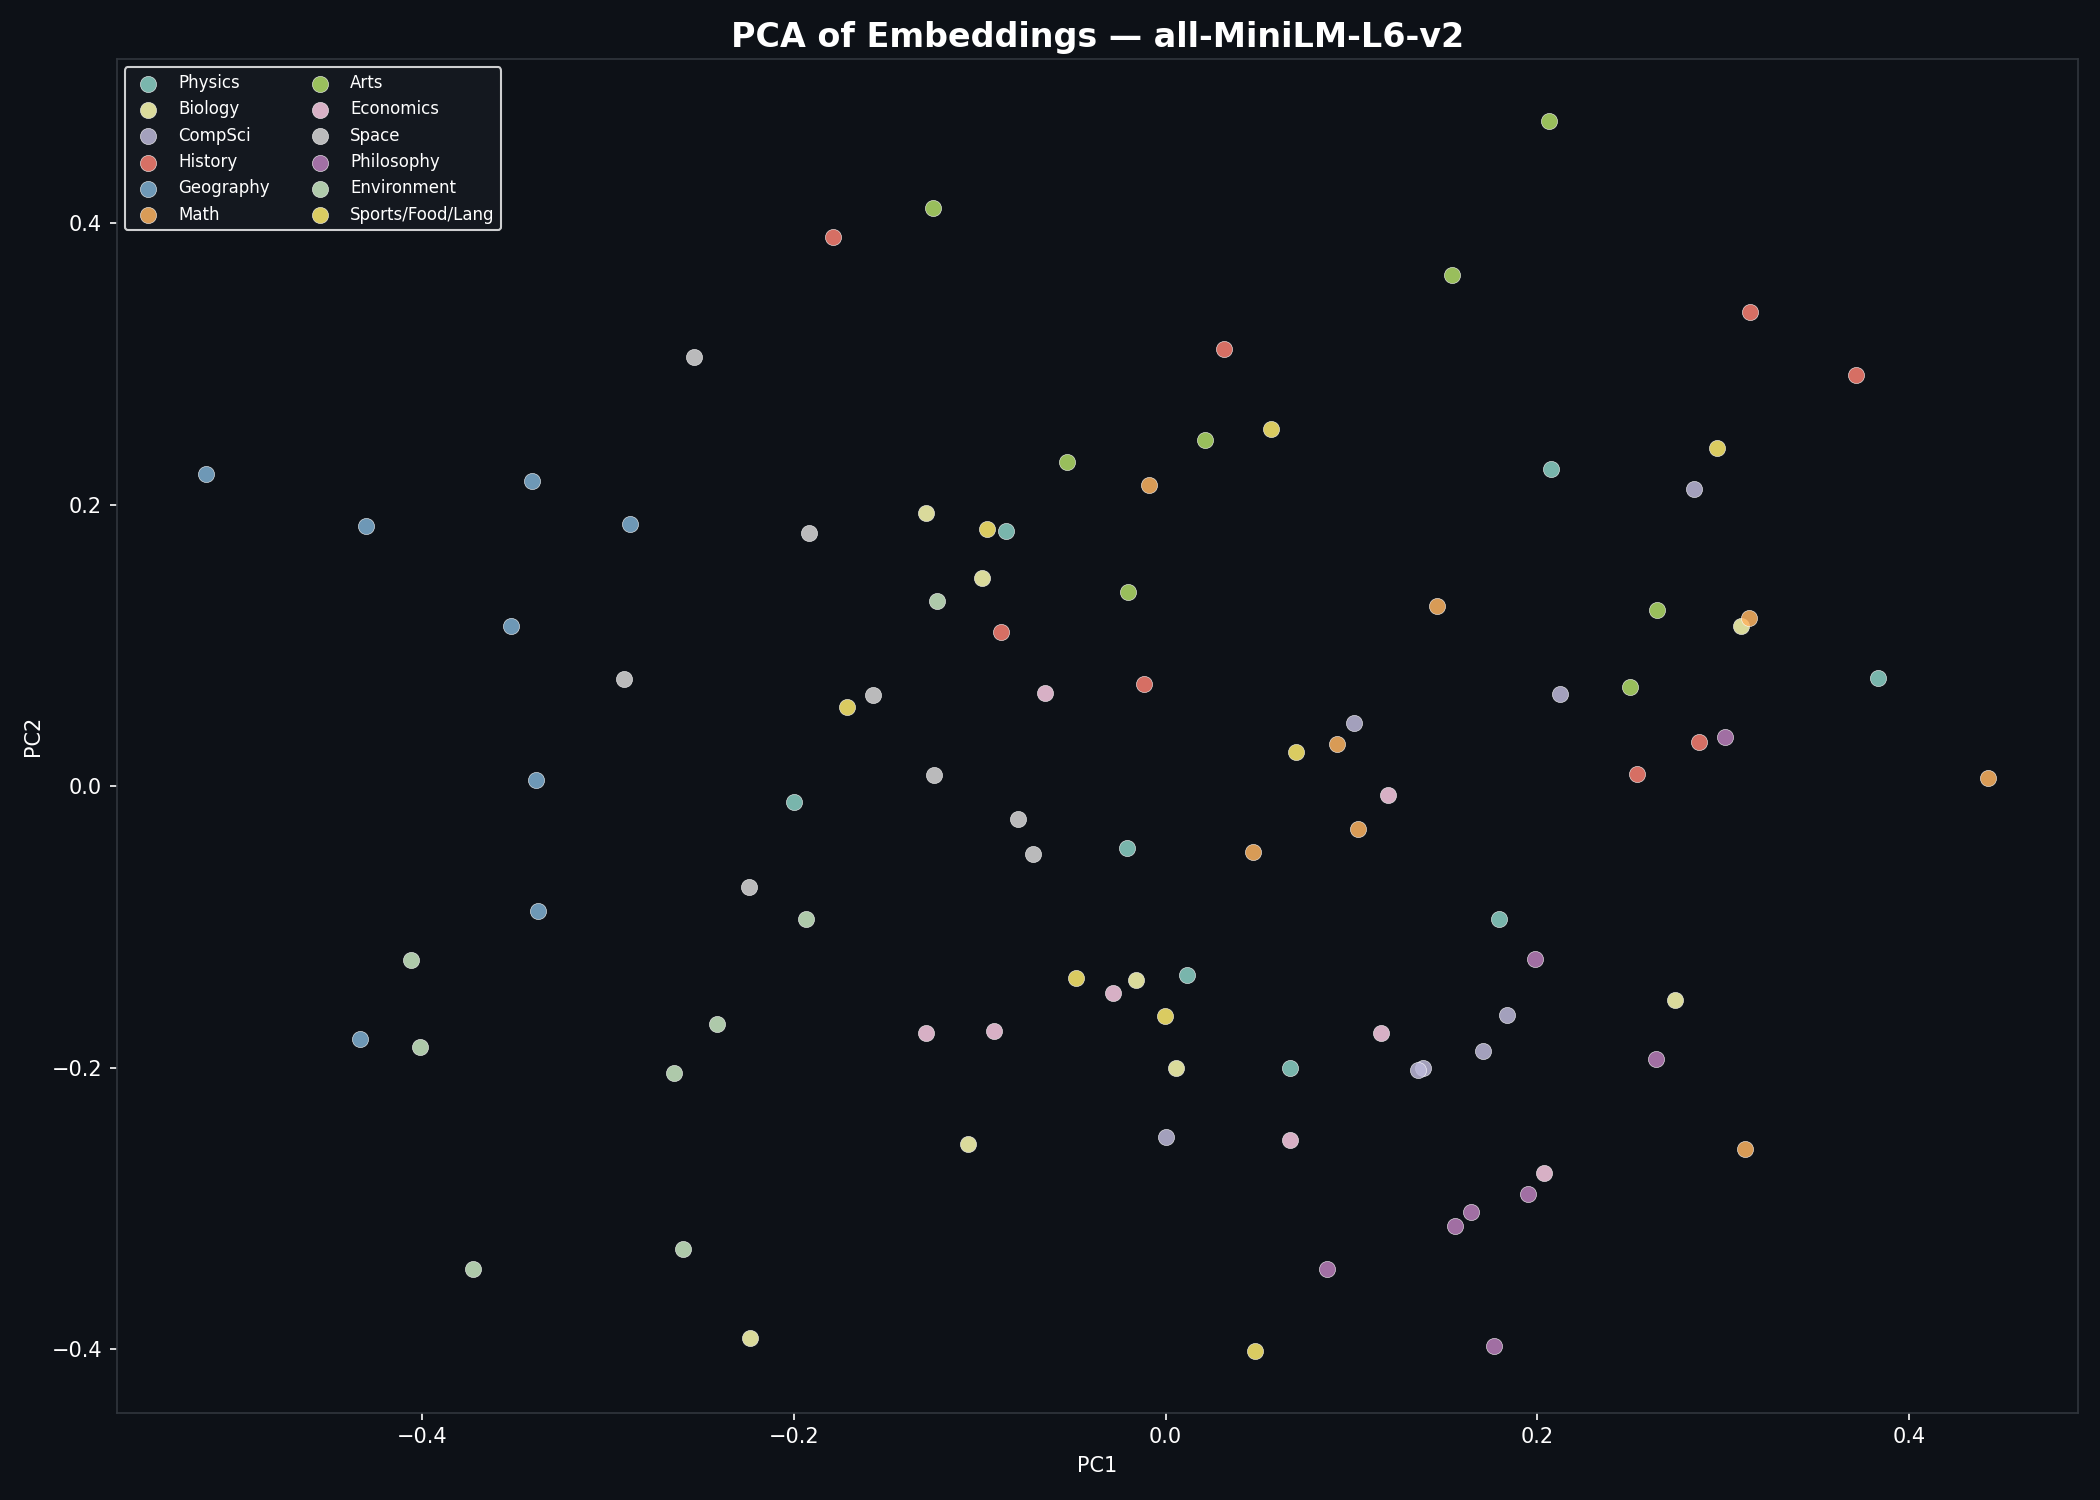
\includegraphics[width=\linewidth]{screenshots/Week3/Lab-3.1-5.png}
        \caption{2D PCA Visualization of Embeddings}
    \end{minipage}
\end{figure}

\vspace{0.5cm}

\subsection{Lab 3.2: Naive RAG Pipeline}
Constructed a standard Retrieval-Augmented Generation pipeline to learn baseline architectures.
\begin{itemize}[label=\textcolor{secondary}{$\bullet$}]
    \item \textbf{Data Ingestion:} Processed 50 pages of PDF content, evaluating the impact of chunk sizes (256 vs 512 vs 1024 tokens) on context retrieval limits.
    \item \textbf{ChromaDB Persistence:} Set up local vector storage indexing metadata alongside page contents for rudimentary filtering.
\end{itemize}

\begin{figure}[H]
    \centering
    \begin{minipage}{0.48\textwidth}
        \centering
        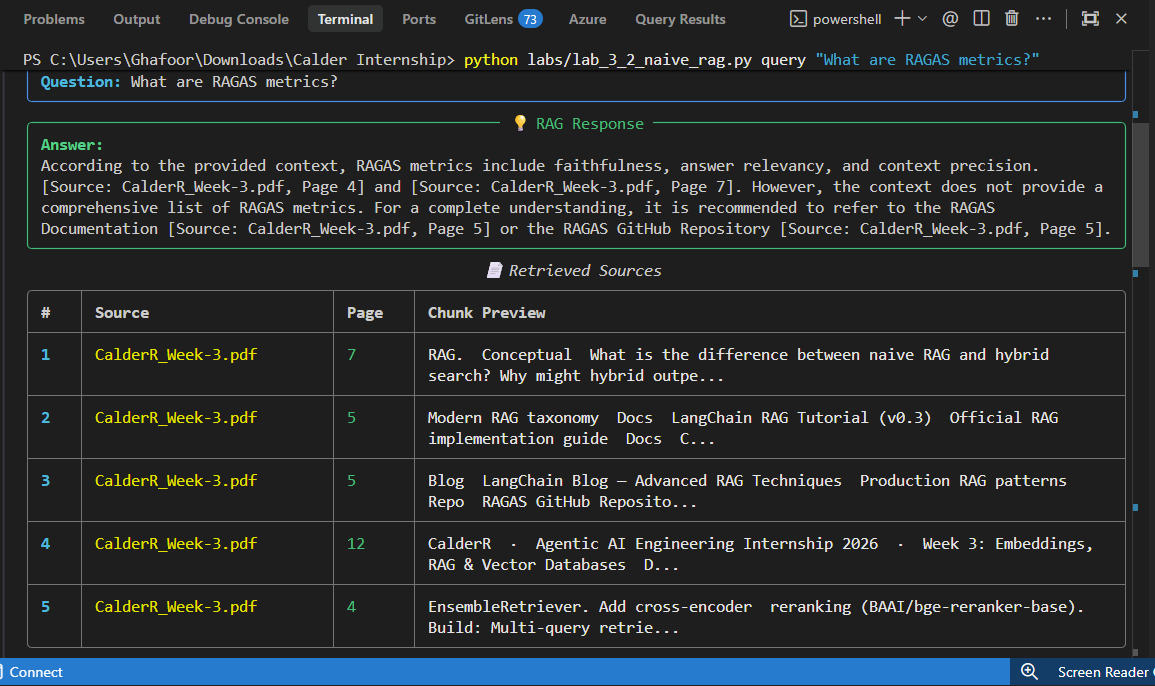
\includegraphics[width=\linewidth]{screenshots/Week3/Lab-3.2-1.png}
        \caption{PDF Ingestion and Splitting}
    \end{minipage}\hfill
    \begin{minipage}{0.48\textwidth}
        \centering
        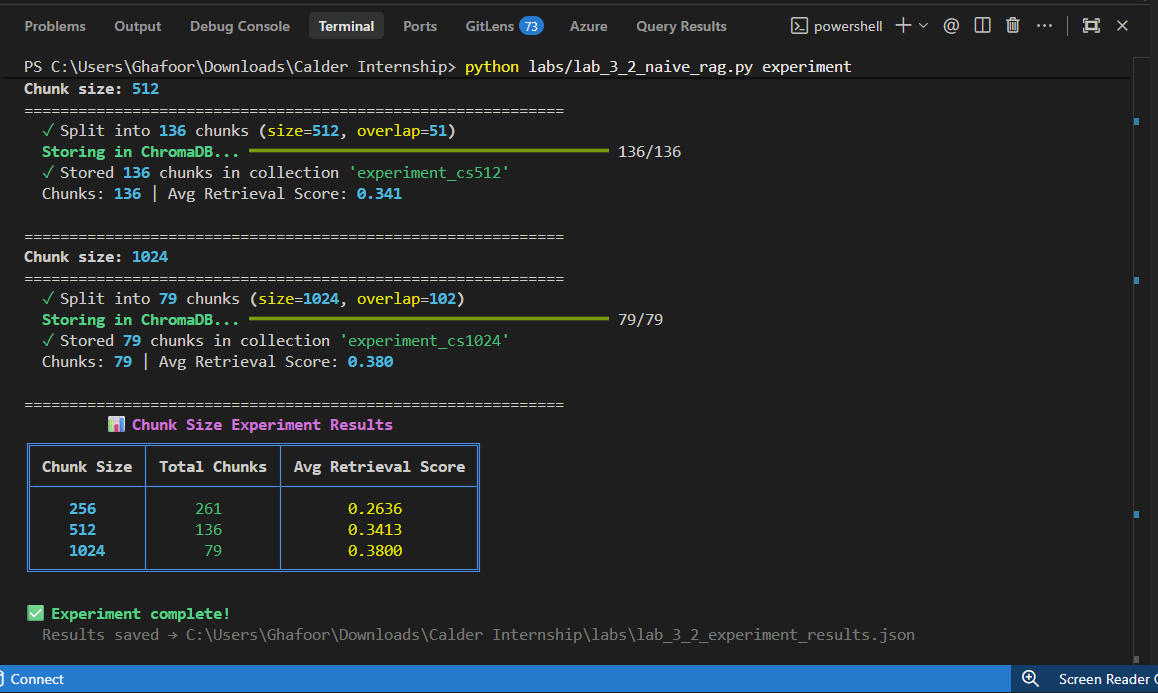
\includegraphics[width=\linewidth]{screenshots/Week3/Lab-3.2-2.png}
        \caption{ChromaDB Indexing and Persistence}
    \end{minipage}
\end{figure}

\begin{figure}[H]
    \centering
    \begin{minipage}{0.5\textwidth}
        \centering
        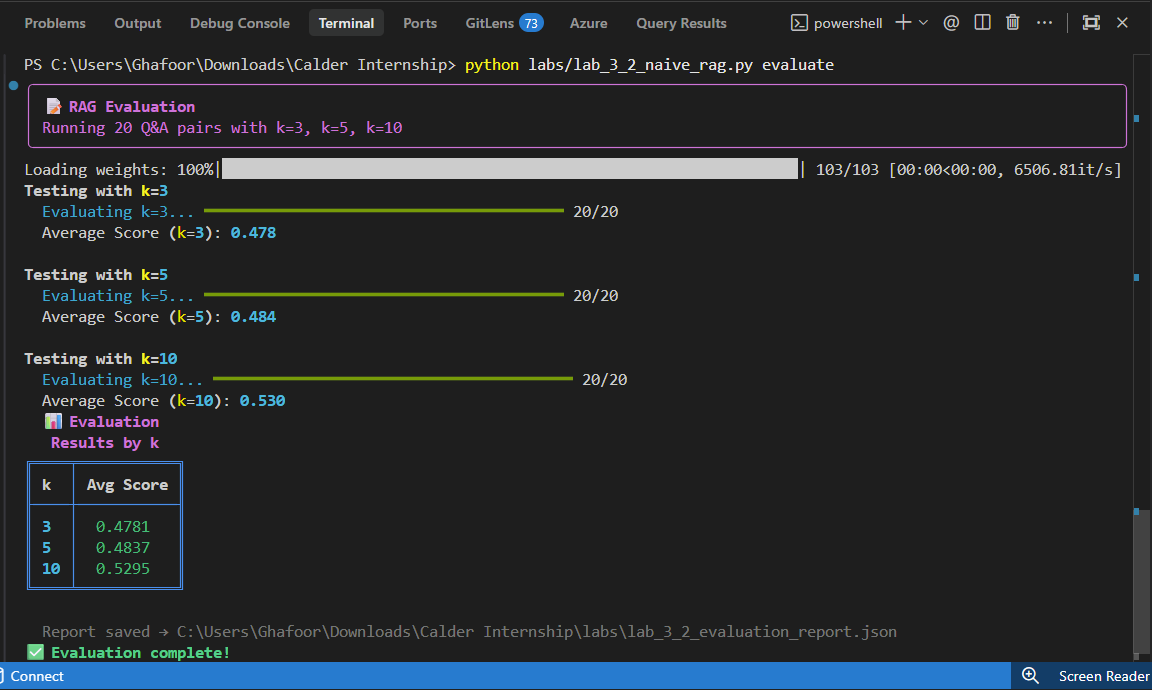
\includegraphics[width=\linewidth]{screenshots/Week3/Lab-3.2-3.png}
        \caption{Naive RAG Answer Generation}
    \end{minipage}
\end{figure}

\newpage

\subsection{Lab 3.3: Hybrid Retrieval \& RAGAS Evaluation}
Graduated from naive RAG to an enterprise-grade retrieval pipeline augmented by mathematical evaluation.
\begin{itemize}[label=\textcolor{secondary}{$\bullet$}]
    \item \textbf{Hybrid Search:} Merged sparse keyword retrieval (BM25) with dense semantic search to eliminate edge cases where users query exact names or IDs.
    \item \textbf{Cross-Encoder Reranking:} Placed a heavy Transformer model right before the LLM to dynamically re-rank the retrieved chunks by highest relevancy.
    \item \textbf{RAGAS Integration:} Formally tested the pipeline's \textit{context precision} and \textit{answer faithfulness} against a golden test dataset.
\end{itemize}

\begin{figure}[H]
    \centering
    \begin{minipage}{0.48\textwidth}
        \centering
        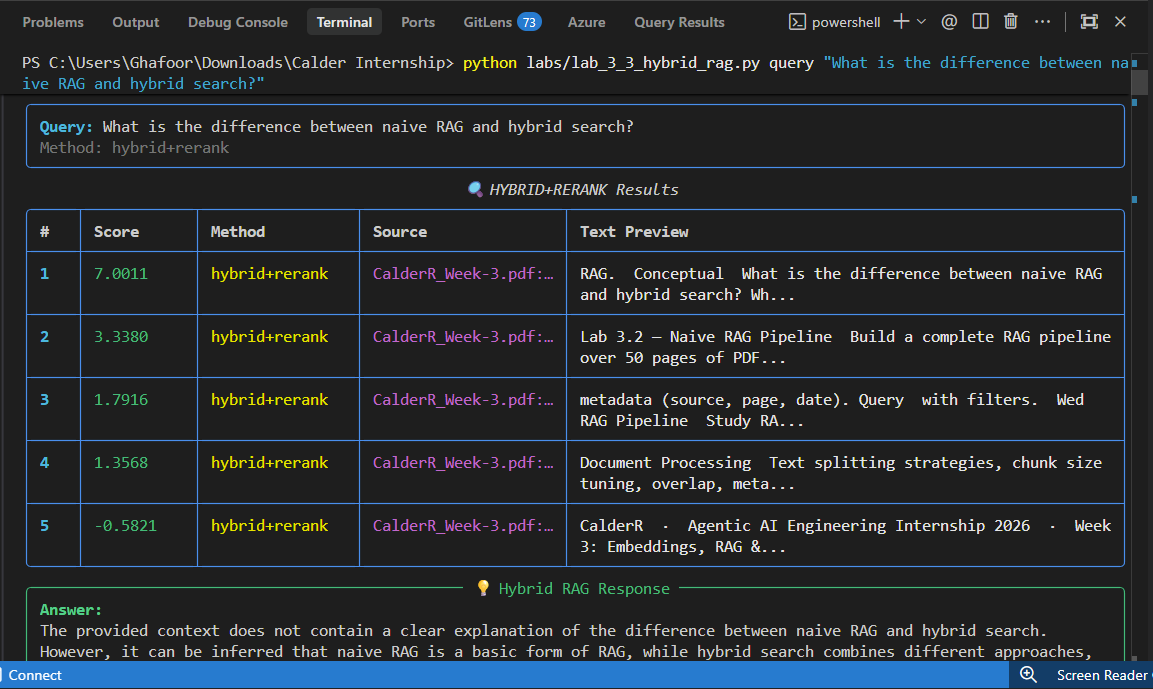
\includegraphics[width=\linewidth]{screenshots/Week3/Lab-3.3-1.png}
        \caption{BM25 + Semantic Hybrid Search}
    \end{minipage}\hfill
    \begin{minipage}{0.48\textwidth}
        \centering
        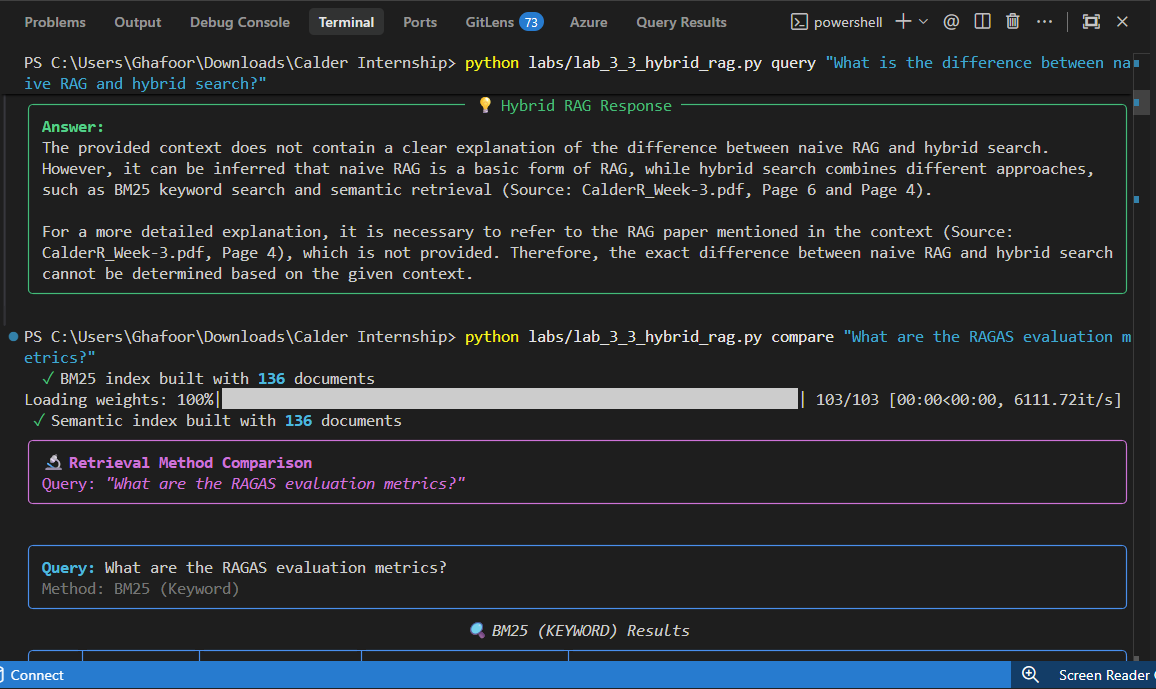
\includegraphics[width=\linewidth]{screenshots/Week3/Lab-3.3-2.png}
        \caption{Cross-Encoder Reranking Execution}
    \end{minipage}
\end{figure}

\begin{figure}[H]
    \centering
    \begin{minipage}{0.48\textwidth}
        \centering
        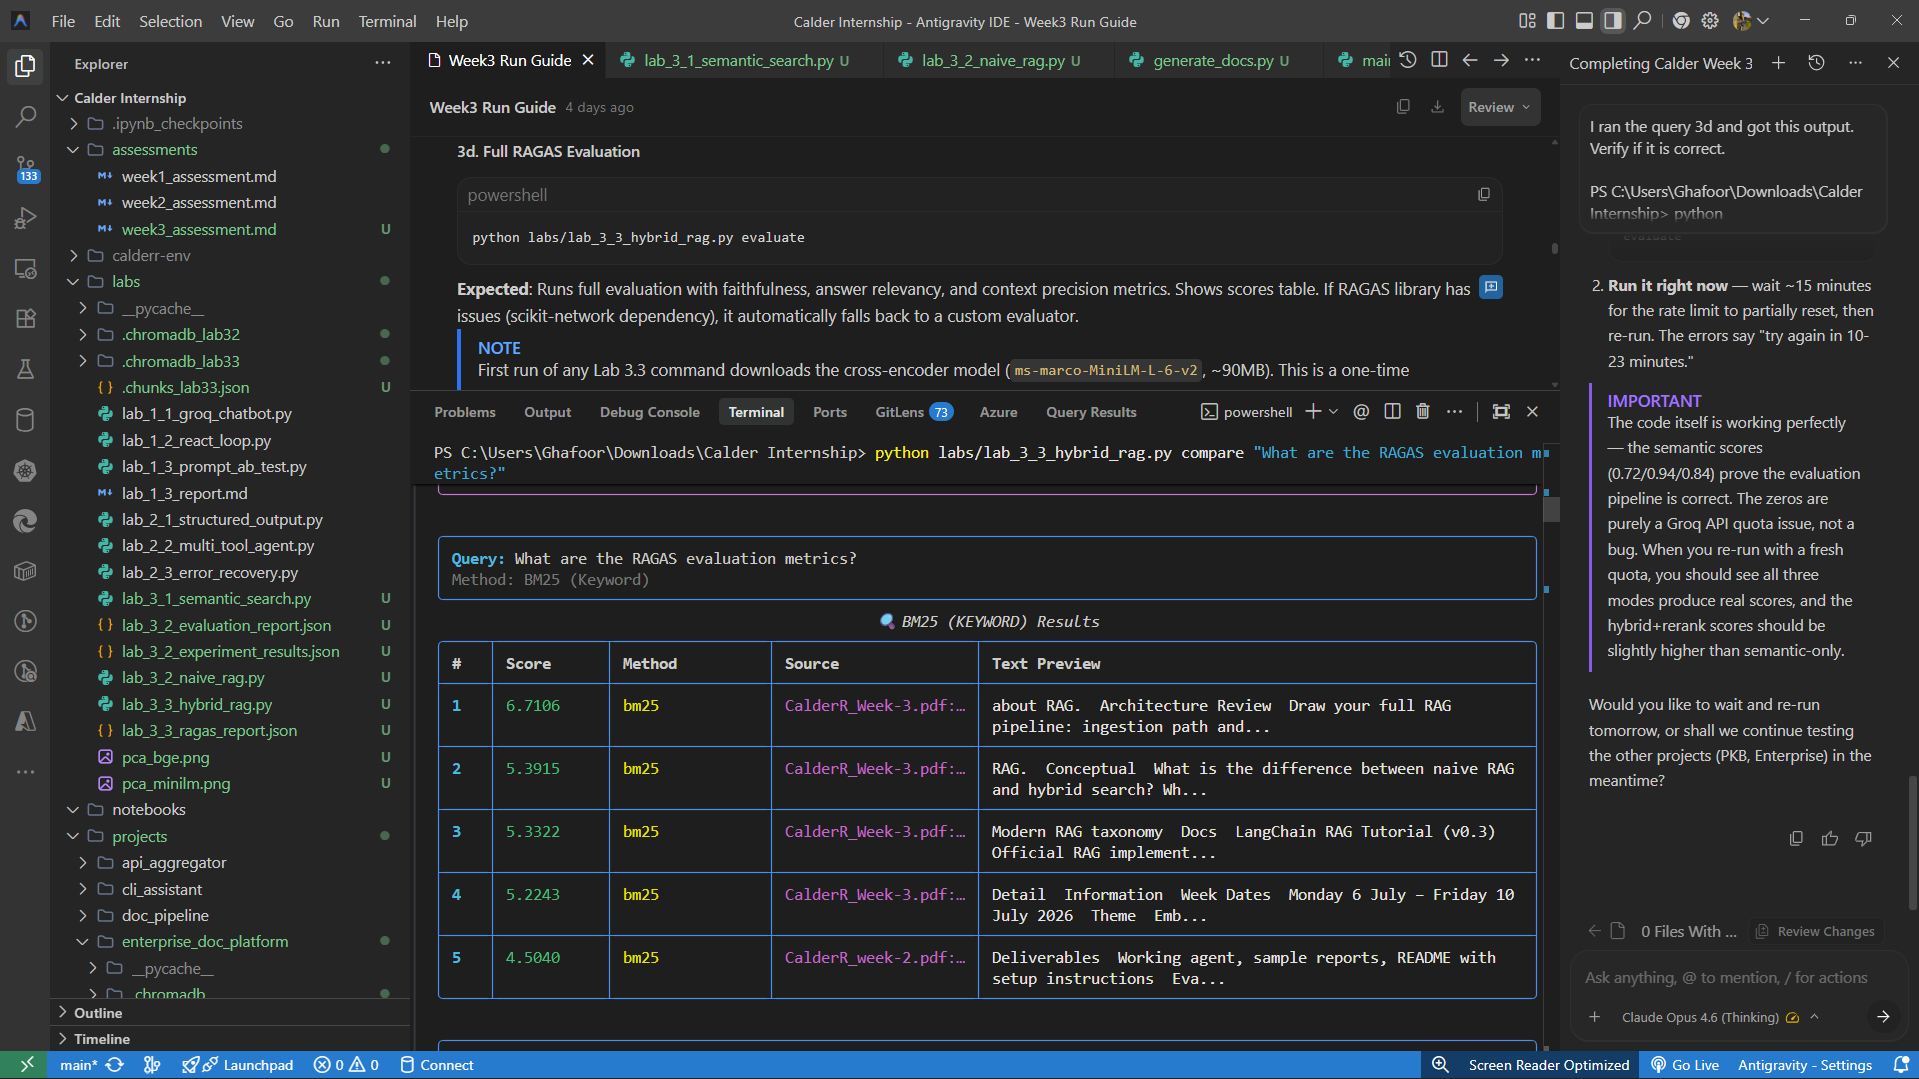
\includegraphics[width=\linewidth]{screenshots/Week3/Lab-3.3-3.png}
        \caption{RAGAS Evaluation Setup}
    \end{minipage}\hfill
    \begin{minipage}{0.48\textwidth}
        \centering
        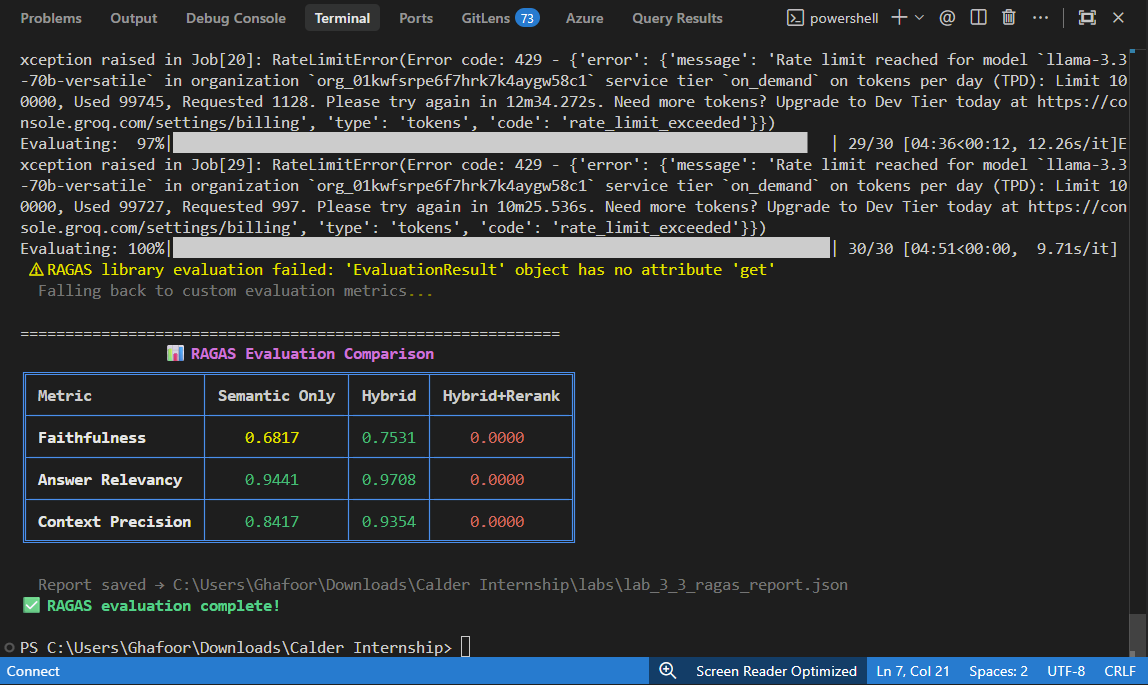
\includegraphics[width=\linewidth]{screenshots/Week3/Lab-3.3-4.png}
        \caption{Generated Context Precision Scores}
    \end{minipage}
\end{figure}

\vspace{0.5cm}

% --- Conclusion ---
\section{Conclusion \& Next Steps}
Week 3 successfully expanded the theoretical reasoning frameworks built previously into tangible, knowledge-aware AI systems. By deeply exploring the mathematics of vector embeddings, mastering local and scalable vector databases like ChromaDB, and engineering sophisticated Hybrid and Cross-Encoder retrieval pipelines, the groundwork for handling complex external data has been solidified. Furthermore, the integration of RAGAS provided a vital engineering capability: the ability to empirically measure LLM application performance rather than relying on subjective "vibe checks."

Moving into the final stages of the internship, the focus will shift towards large-scale orchestration, autonomous multi-agent systems, and deploying stateful graphs that combine our knowledge bases with complex tool-calling workflows.

\end{document}
